%========================================================================
\section{Results and Interpretation}\label{sec:results}
%========================================================================

\subsection{Linear feature reduction}
\textbf{PCA.} On the standardised 80{,}000-row training matrix the first two principal components explain 17.5\% and 14.9\% of the variance, and \textbf{16 of the 25 components} are needed to reach 95\% (Fig.~\ref{fig:pca}). This flat spectrum is typical of noisy, weakly correlated data. The last four components carry essentially zero variance because \texttt{Type\_A}+\texttt{Type\_B}+\texttt{Type\_C}$=1$ and because \texttt{Week}, \texttt{Days\_to\_Thanksgiving} and \texttt{Days\_to\_Christmas} are exact linear functions of each other within a year, which confirms the redundancy noted in Section~\ref{sec:data}. The loadings are easy to interpret: PC1 is a \emph{seasonality} axis (equal loadings of 0.43 on \texttt{Week}, \texttt{Month} and the two days-to-holiday variables), and PC2 is a \emph{promotion-era} axis (\texttt{MarkDown\_Available} 0.41, \texttt{MarkDown5} 0.37, \texttt{MarkDown1} 0.36, \texttt{Year} 0.34). Neither axis involves \texttt{Dept} or \texttt{Size}, the two most predictive features, so the variance-maximising view of the data is largely orthogonal to the sales-level question. In Fig.~\ref{fig:linear} the PCA projection therefore shows clear structure --- parallel bands along the seasonal and promotion-era axes --- but the three classes are completely mixed.

\textbf{LDA.} Because it uses the labels, LDA is the only linear method that targets class separation. The first discriminant explains 84.3\% of the between-class variance. In the 2-D LDA map a Low-dominated region and a High-dominated region become visible, and the 5-NN accuracy in the embedding is the best of all ten 2-D maps (46.3\%; Table~\ref{tab:emb}). Used directly as a linear classifier, however, LDA reaches only 44.1\% test accuracy. The class boundaries are therefore not linear in the original features, which foreshadows the poor results of the linear classifiers in Section~\ref{sec:res:models}.

\textbf{SVD.} Truncated SVD on standardised (hence centred) data reproduces the PCA solution up to sign: the explained-variance ratios of the first two components (17.4\% and 15.0\%), the 5-NN accuracy (37.1\%) and the trustworthiness (0.889) are identical to PCA's within rounding. The leading singular values are 591.7, 545.4, 447.6, 392.6 and 375.9. This sanity check confirms the equivalence $\mathbf{X}=\mathbf{U}\boldsymbol{\Sigma}\mathbf{V}^\top\Rightarrow\mathbf{C}=\mathbf{V}\frac{\boldsymbol{\Sigma}^2}{n-1}\mathbf{V}^\top$ for centred $\mathbf{X}$.

\begin{figure*}[!t]
\centering
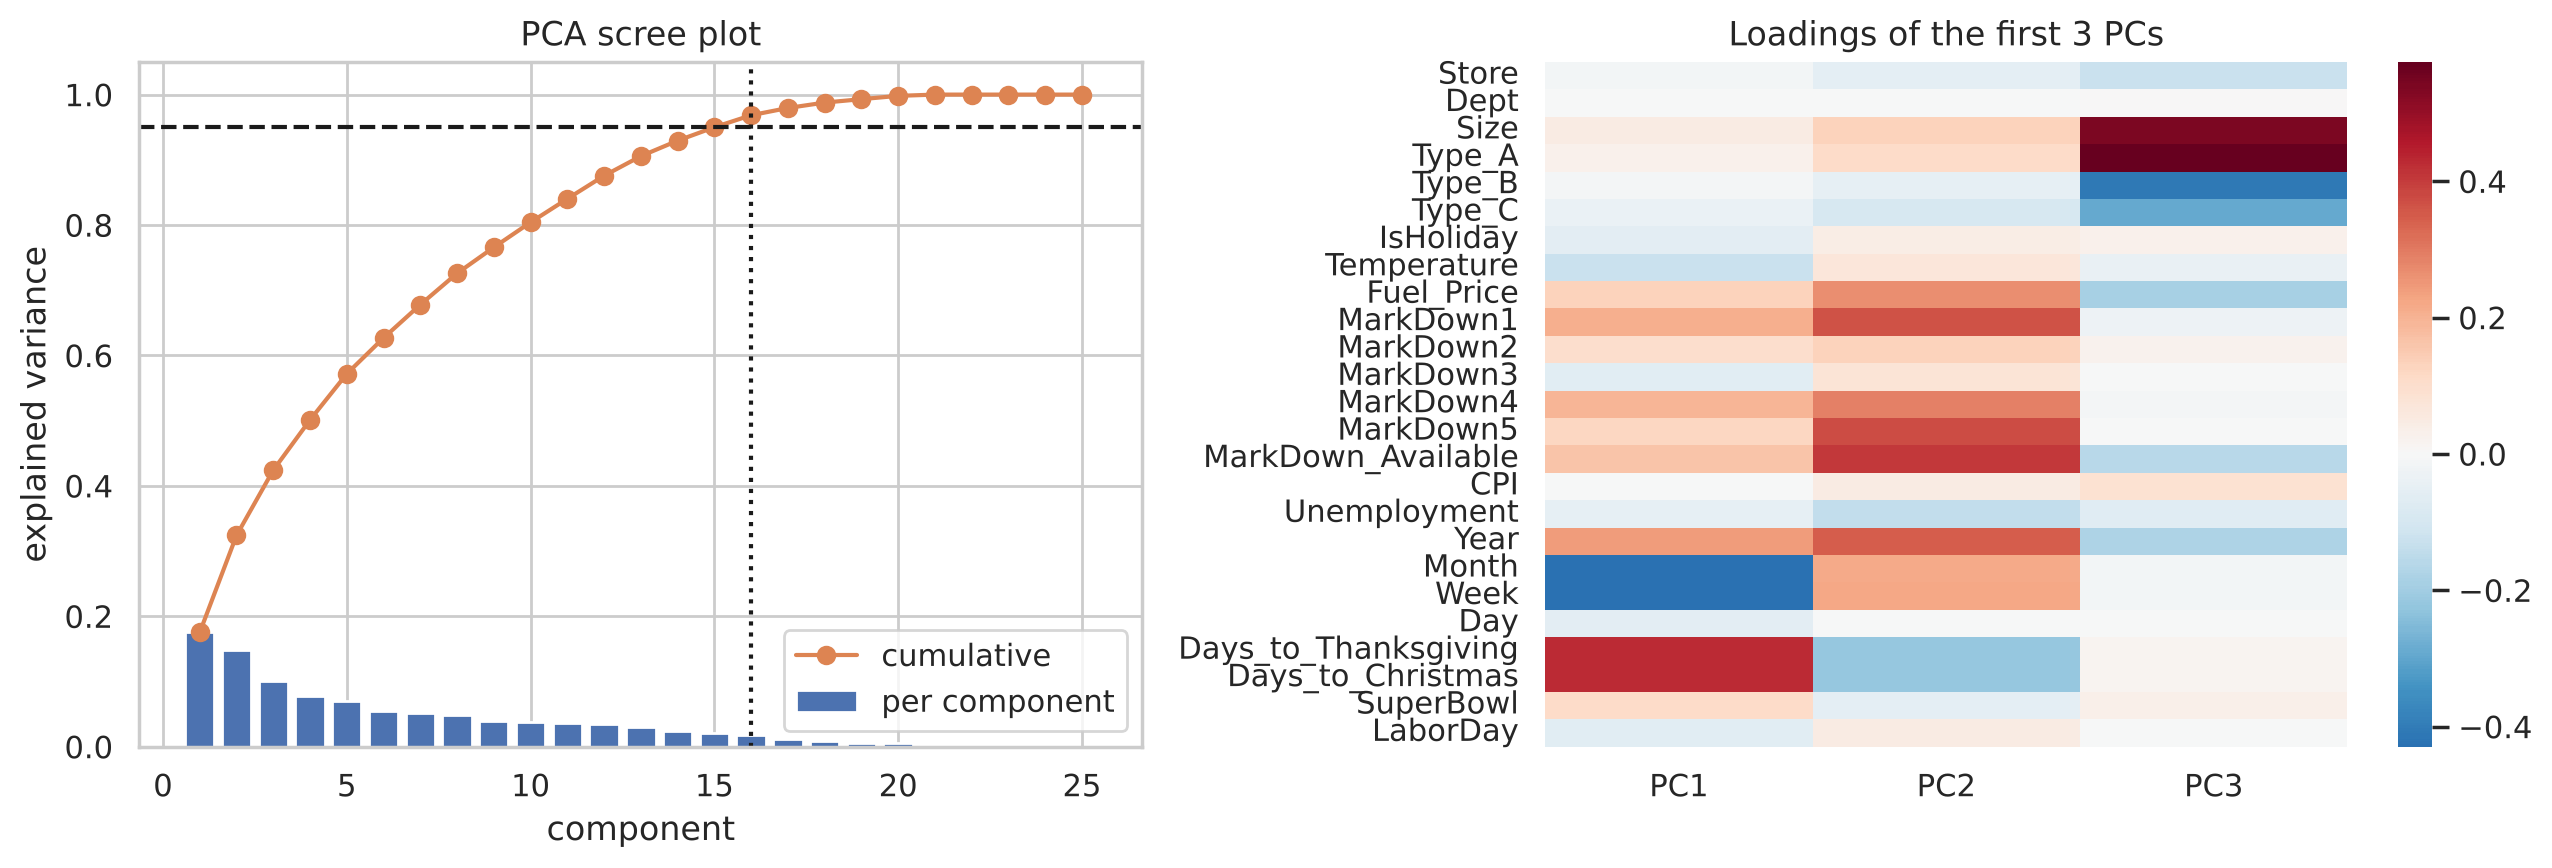
\includegraphics[width=0.85\textwidth]{figures/04_pca_scree_loadings.png}
\caption{PCA on the training split. Left: scree plot with the cumulative explained variance (16 components reach 95\%). Right: loadings of the first three components --- PC1 is seasonality, PC2 is the promotion era.}
\label{fig:pca}
\end{figure*}

\begin{figure*}[!t]
\centering
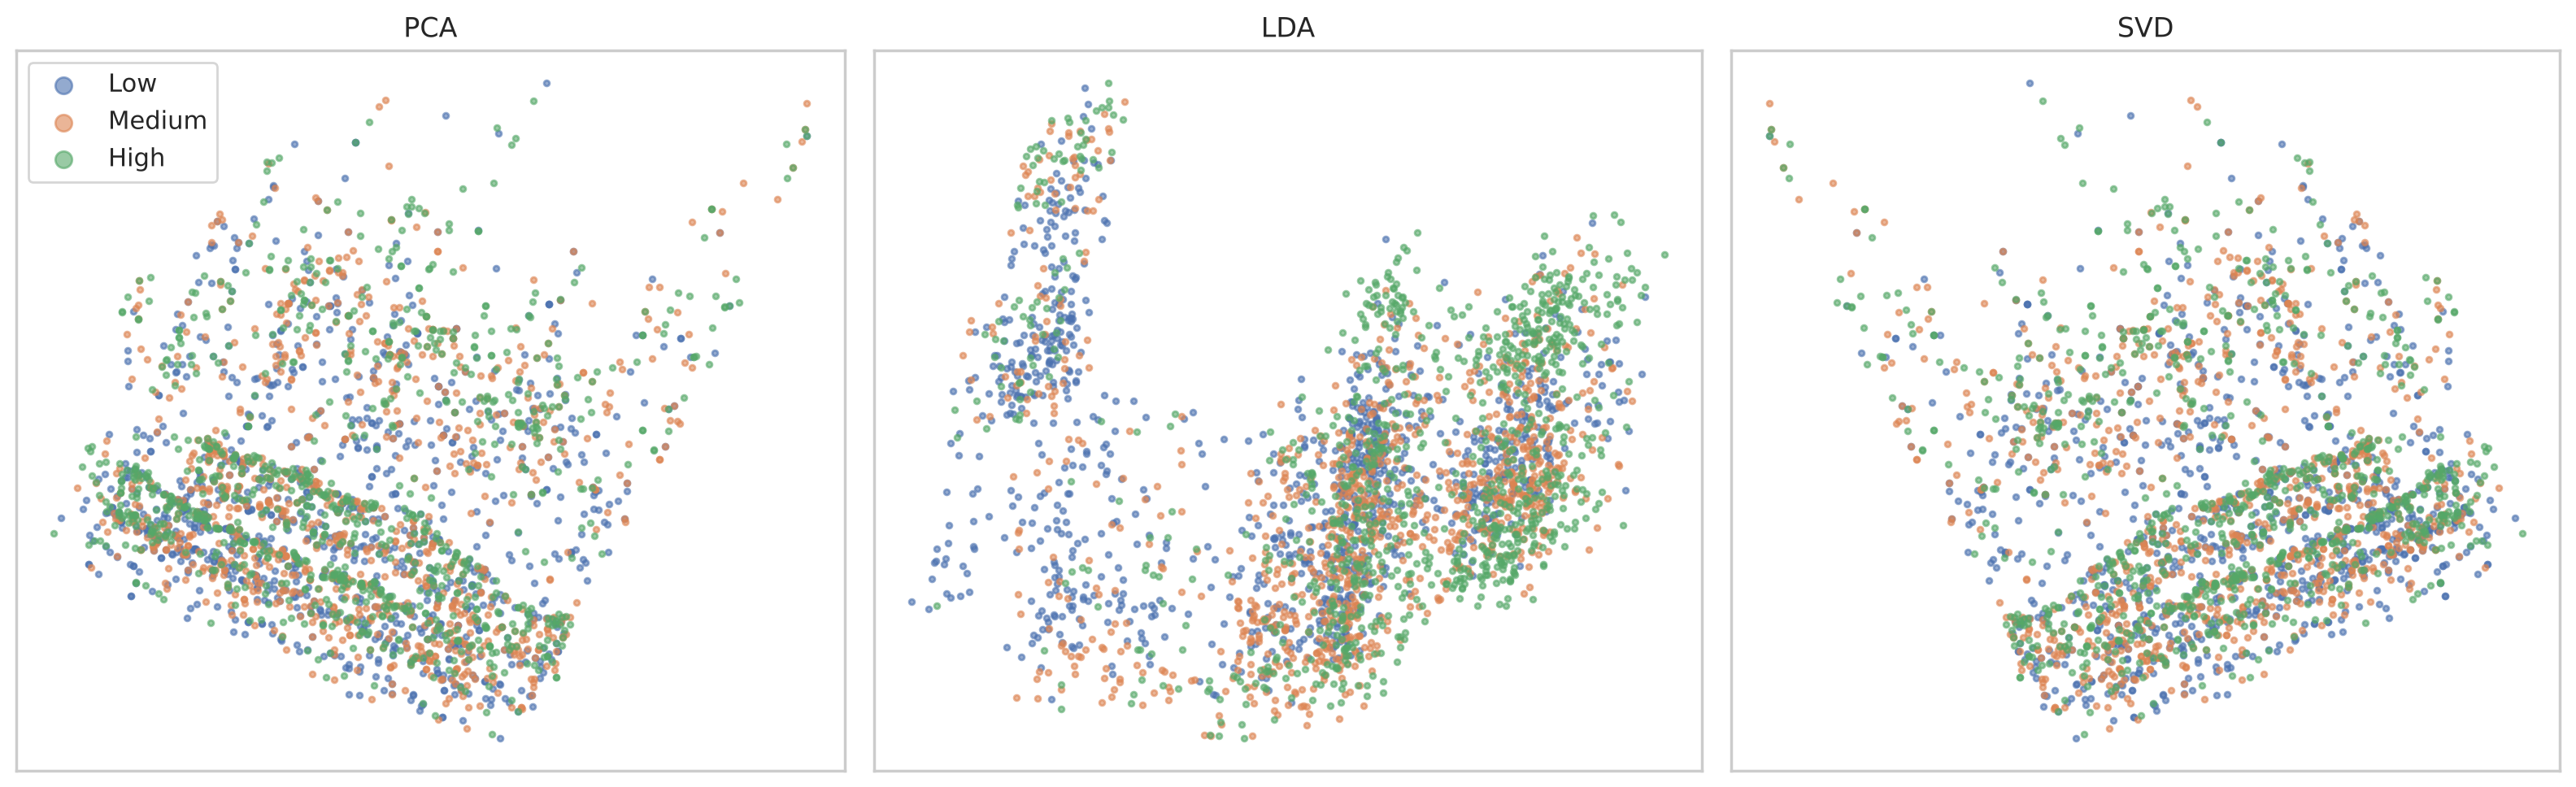
\includegraphics[width=0.92\textwidth]{figures/05_linear_embeddings.png}
\caption{Linear 2-D embeddings of the 3{,}000-point visualisation sample, coloured by the true sales class. PCA and SVD are identical up to sign; only the supervised LDA shows partial class separation.}
\label{fig:linear}
\end{figure*}

\subsection{Non-linear feature reduction}
Table~\ref{tab:emb} and Fig.~\ref{fig:allemb} compare all ten embeddings. Three different patterns appear.

\emph{Neighbourhood preservation.} t-SNE (trustworthiness 0.996) and UMAP (0.990) preserve local neighbourhoods almost perfectly, followed by our SNE implementation (0.958). The global methods --- PCA, SVD, Kernel PCA, both MDS variants and Isomap --- lie between 0.89 and 0.91, and LLE is lowest (0.841). This ranking matches theory: the neighbour-embedding family optimises exactly what trustworthiness measures, whereas distance-preserving methods trade local fidelity for global layout. In the t-SNE and UMAP maps the data split into a handful of compact islands. To find out what they represent, we trained a 5-NN classifier in each embedding to predict different labels. It recovers the store type with 99.4\% (t-SNE) and 98.8\% (UMAP) accuracy, the year with 97.8\% and 96.3\%, and the promotion era (\texttt{MarkDown\_Available}) with 99.5\% and 99.3\%, but the sales class with only 39.5\% and 38.8\%. The islands are therefore \emph{store-context} groups (type $\times$ year $\times$ promotion regime), not sales segments.

\emph{Class information.} No unsupervised embedding separates the classes well. The 5-NN accuracies lie between 35.1\% (LLE) and 39.5\% (t-SNE), all \emph{below} the 41.2\% obtained by 5-NN on the 25 standardised features themselves. All class silhouettes are slightly negative ($-0.08$ to $-0.01$), meaning that a point is on average as close to points of the other classes as to its own. Squeezing 25 noisy dimensions into two therefore loses class information, and the loss is largest for methods whose objective is global (MDS, Isomap) or fragile (LLE). LDA is the exception because it is supervised.

\emph{Method-specific behaviour.} \textbf{Kernel PCA} performed best with the smallest bandwidth tried ($\gamma=0.005$), where the RBF kernel is almost linear, and is then visually and numerically close to PCA (36.4\%). Larger $\gamma$ values produced numerically unstable eigenvectors and were discarded. \textbf{SNE} produces a looser, more uniform cloud than t-SNE --- the classic \emph{crowding problem} that motivated the heavy-tailed kernel of t-SNE~\cite{vandermaaten2008} --- and it is also by far the slowest method in our pure-NumPy implementation (44.8\,s for 1{,}500 points, against 7.9\,s for t-SNE on 3{,}000 points). \textbf{Metric and non-metric MDS} give nearly identical maps (37.4\% and 37.0\%). The rank-based non-metric variant costs 14 times more (55.2\,s versus 4.0\,s) for no benefit, which shows that the distance structure contains no monotone distortion worth modelling. \textbf{Isomap} unrolls the data into elongated filaments that follow the calendar ordering. \textbf{LLE} collapses most points onto a single line (Fig.~\ref{fig:allemb}). This is a well-known failure mode when the neighbourhood graph contains many exact duplicates: here, departments of the same store-week share every context feature, so the local reconstruction problem becomes degenerate.

\begin{table}[!t]
\caption{Quality of the 2-D embeddings (3{,}000-point training sample). kNN = 5-fold 5-NN accuracy in the embedding; reference on the 25 raw standardised features: 0.412}
\label{tab:emb}
\centering
\setlength{\tabcolsep}{4pt}
\begin{tabular}{lcccr}
\toprule
Method & kNN acc. & Trustw. & Class sil. & Time (s) \\
\midrule
\multicolumn{5}{l}{\emph{Linear}}\\
PCA & 0.371 & 0.889 & $-0.016$ & 0.002 \\
LDA (supervised) & \textbf{0.463} & 0.699 & $-0.020$ & 0.14 \\
SVD & 0.371 & 0.889 & $-0.016$ & 0.005 \\
\midrule
\multicolumn{5}{l}{\emph{Non-linear}}\\
Kernel PCA ($\gamma$=0.005) & 0.364 & 0.889 & $-0.014$ & 2.1 \\
SNE$^\dagger$ & 0.373 & 0.958 & $-0.019$ & 44.8 \\
t-SNE & 0.395 & \textbf{0.996} & $-0.024$ & 7.9 \\
UMAP & 0.388 & 0.990 & $-0.030$ & 10.8 \\
Metric MDS$^\ddagger$ & 0.374 & 0.899 & $-0.023$ & 4.0 \\
Non-metric MDS$^\ddagger$ & 0.370 & 0.900 & $-0.029$ & 55.2 \\
Isomap & 0.374 & 0.910 & $-0.043$ & 1.9 \\
LLE & 0.351 & 0.841 & $-0.079$ & 2.3 \\
\bottomrule
\multicolumn{5}{l}{\footnotesize $^\dagger$1{,}500 points, own NumPy implementation; $^\ddagger$1{,}000 points.}
\end{tabular}
\end{table}

\begin{figure*}[!t]
\centering
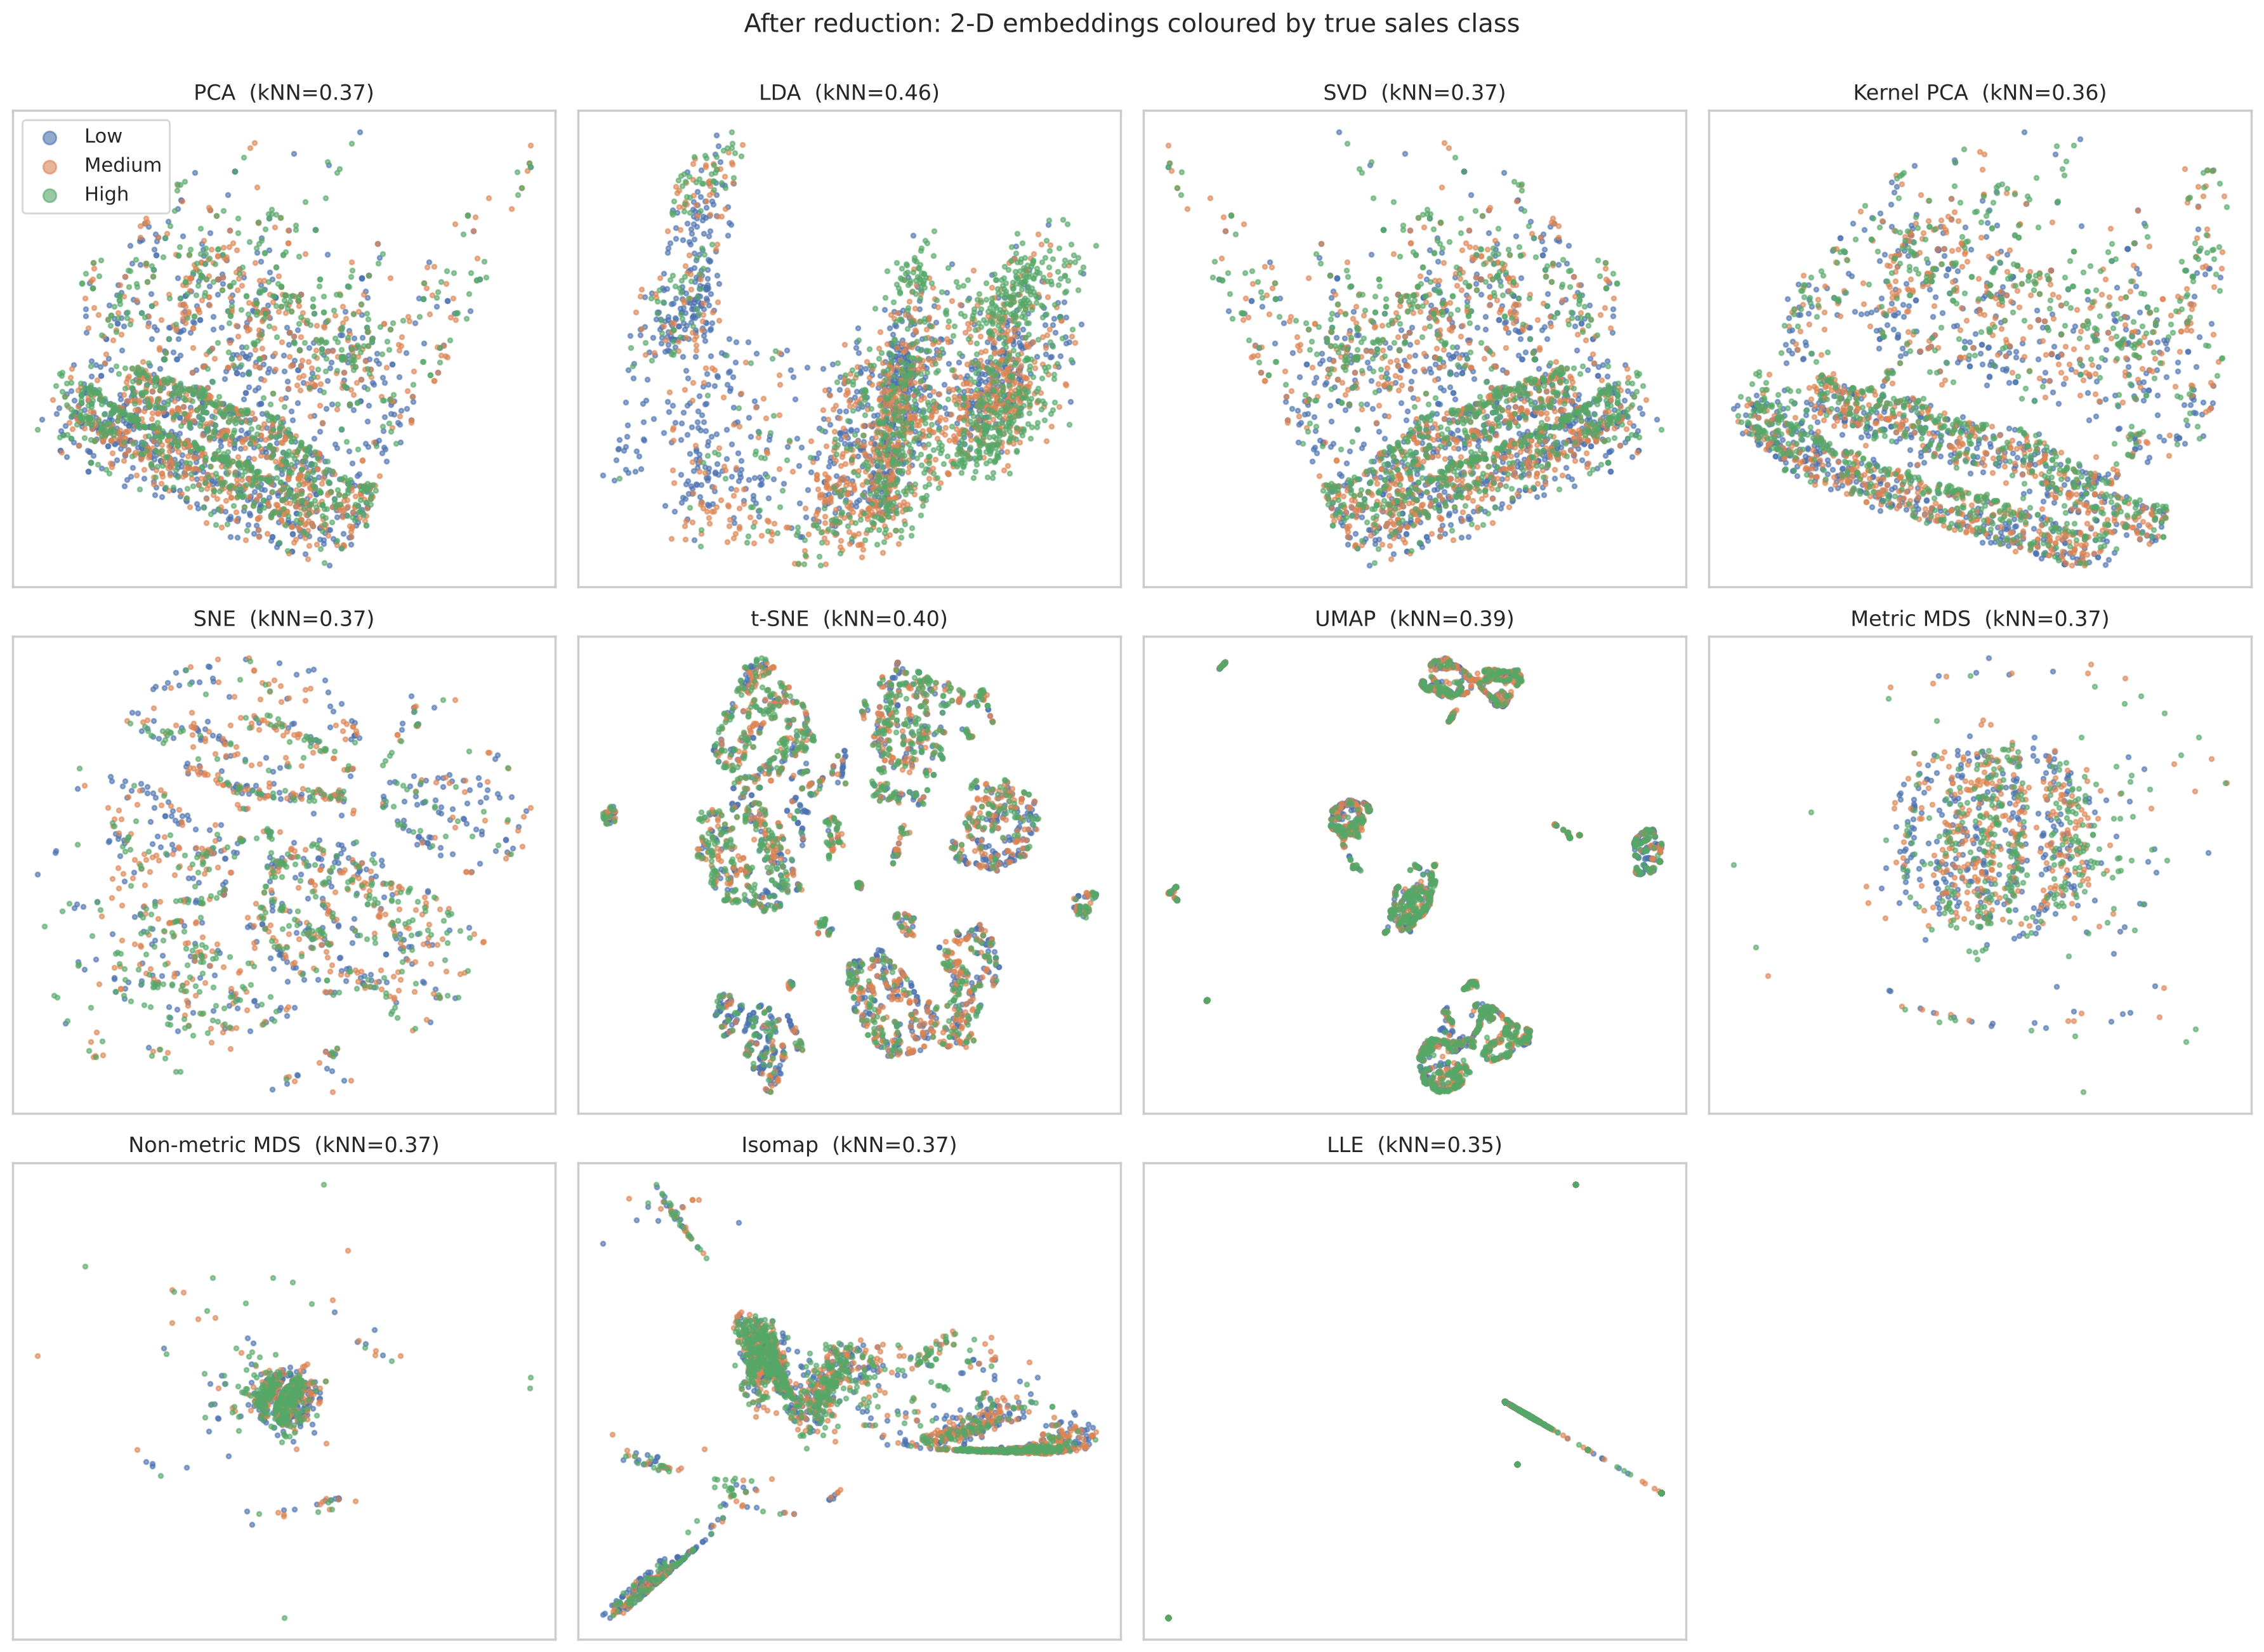
\includegraphics[width=\textwidth]{figures/06_all_embeddings.png}
\caption{After reduction: all ten 2-D embeddings coloured by the true sales class (5-NN accuracy in brackets). Neighbour-embedding methods (t-SNE, UMAP) reveal compact store-context islands, but no unsupervised method separates the sales classes.}
\label{fig:allemb}
\end{figure*}

\subsection{Clustering before and after reduction}
Table~\ref{tab:clu} and Fig.~\ref{fig:clu} report K-Means ($k=3$) in six spaces. In the original 25-D space and in the 16-D PCA space the clusters are weak (silhouette 0.13--0.14). After reduction to 2-D the silhouette rises sharply: 0.44 (PCA), 0.45 (LDA), 0.47 (t-SNE) and 0.57 (UMAP). UMAP's compact islands are exactly what K-Means rewards. The agreement with the true sales classes, however, is close to zero everywhere (ARI $\le0.018$, NMI $\le0.024$). The data clearly contain natural groups --- seasons, promotion eras, store-size tiers --- but these groups are orthogonal to the sales level of a department. This is the central negative result of the unsupervised part of the study: \emph{a high silhouette after reduction does not mean that the clusters are meaningful for the business target}, and an analyst who reads a good-looking UMAP map as ``three sales segments'' would be badly misled.

\begin{table}[!t]
\caption{K-Means ($k=3$) before and after reduction}
\label{tab:clu}
\centering
\begin{tabular}{lccc}
\toprule
Space & Silhouette & ARI & NMI \\
\midrule
Original (25-D) & 0.131 & 0.000 & 0.001 \\
PCA (16-D, 95\% var.) & 0.136 & 0.000 & 0.001 \\
PCA (2-D) & 0.437 & 0.001 & 0.001 \\
LDA (2-D) & 0.453 & \textbf{0.018} & \textbf{0.024} \\
t-SNE (2-D) & 0.473 & 0.008 & 0.008 \\
UMAP (2-D) & \textbf{0.570} & 0.009 & 0.009 \\
\bottomrule
\end{tabular}
\end{table}

\begin{figure*}[!t]
\centering
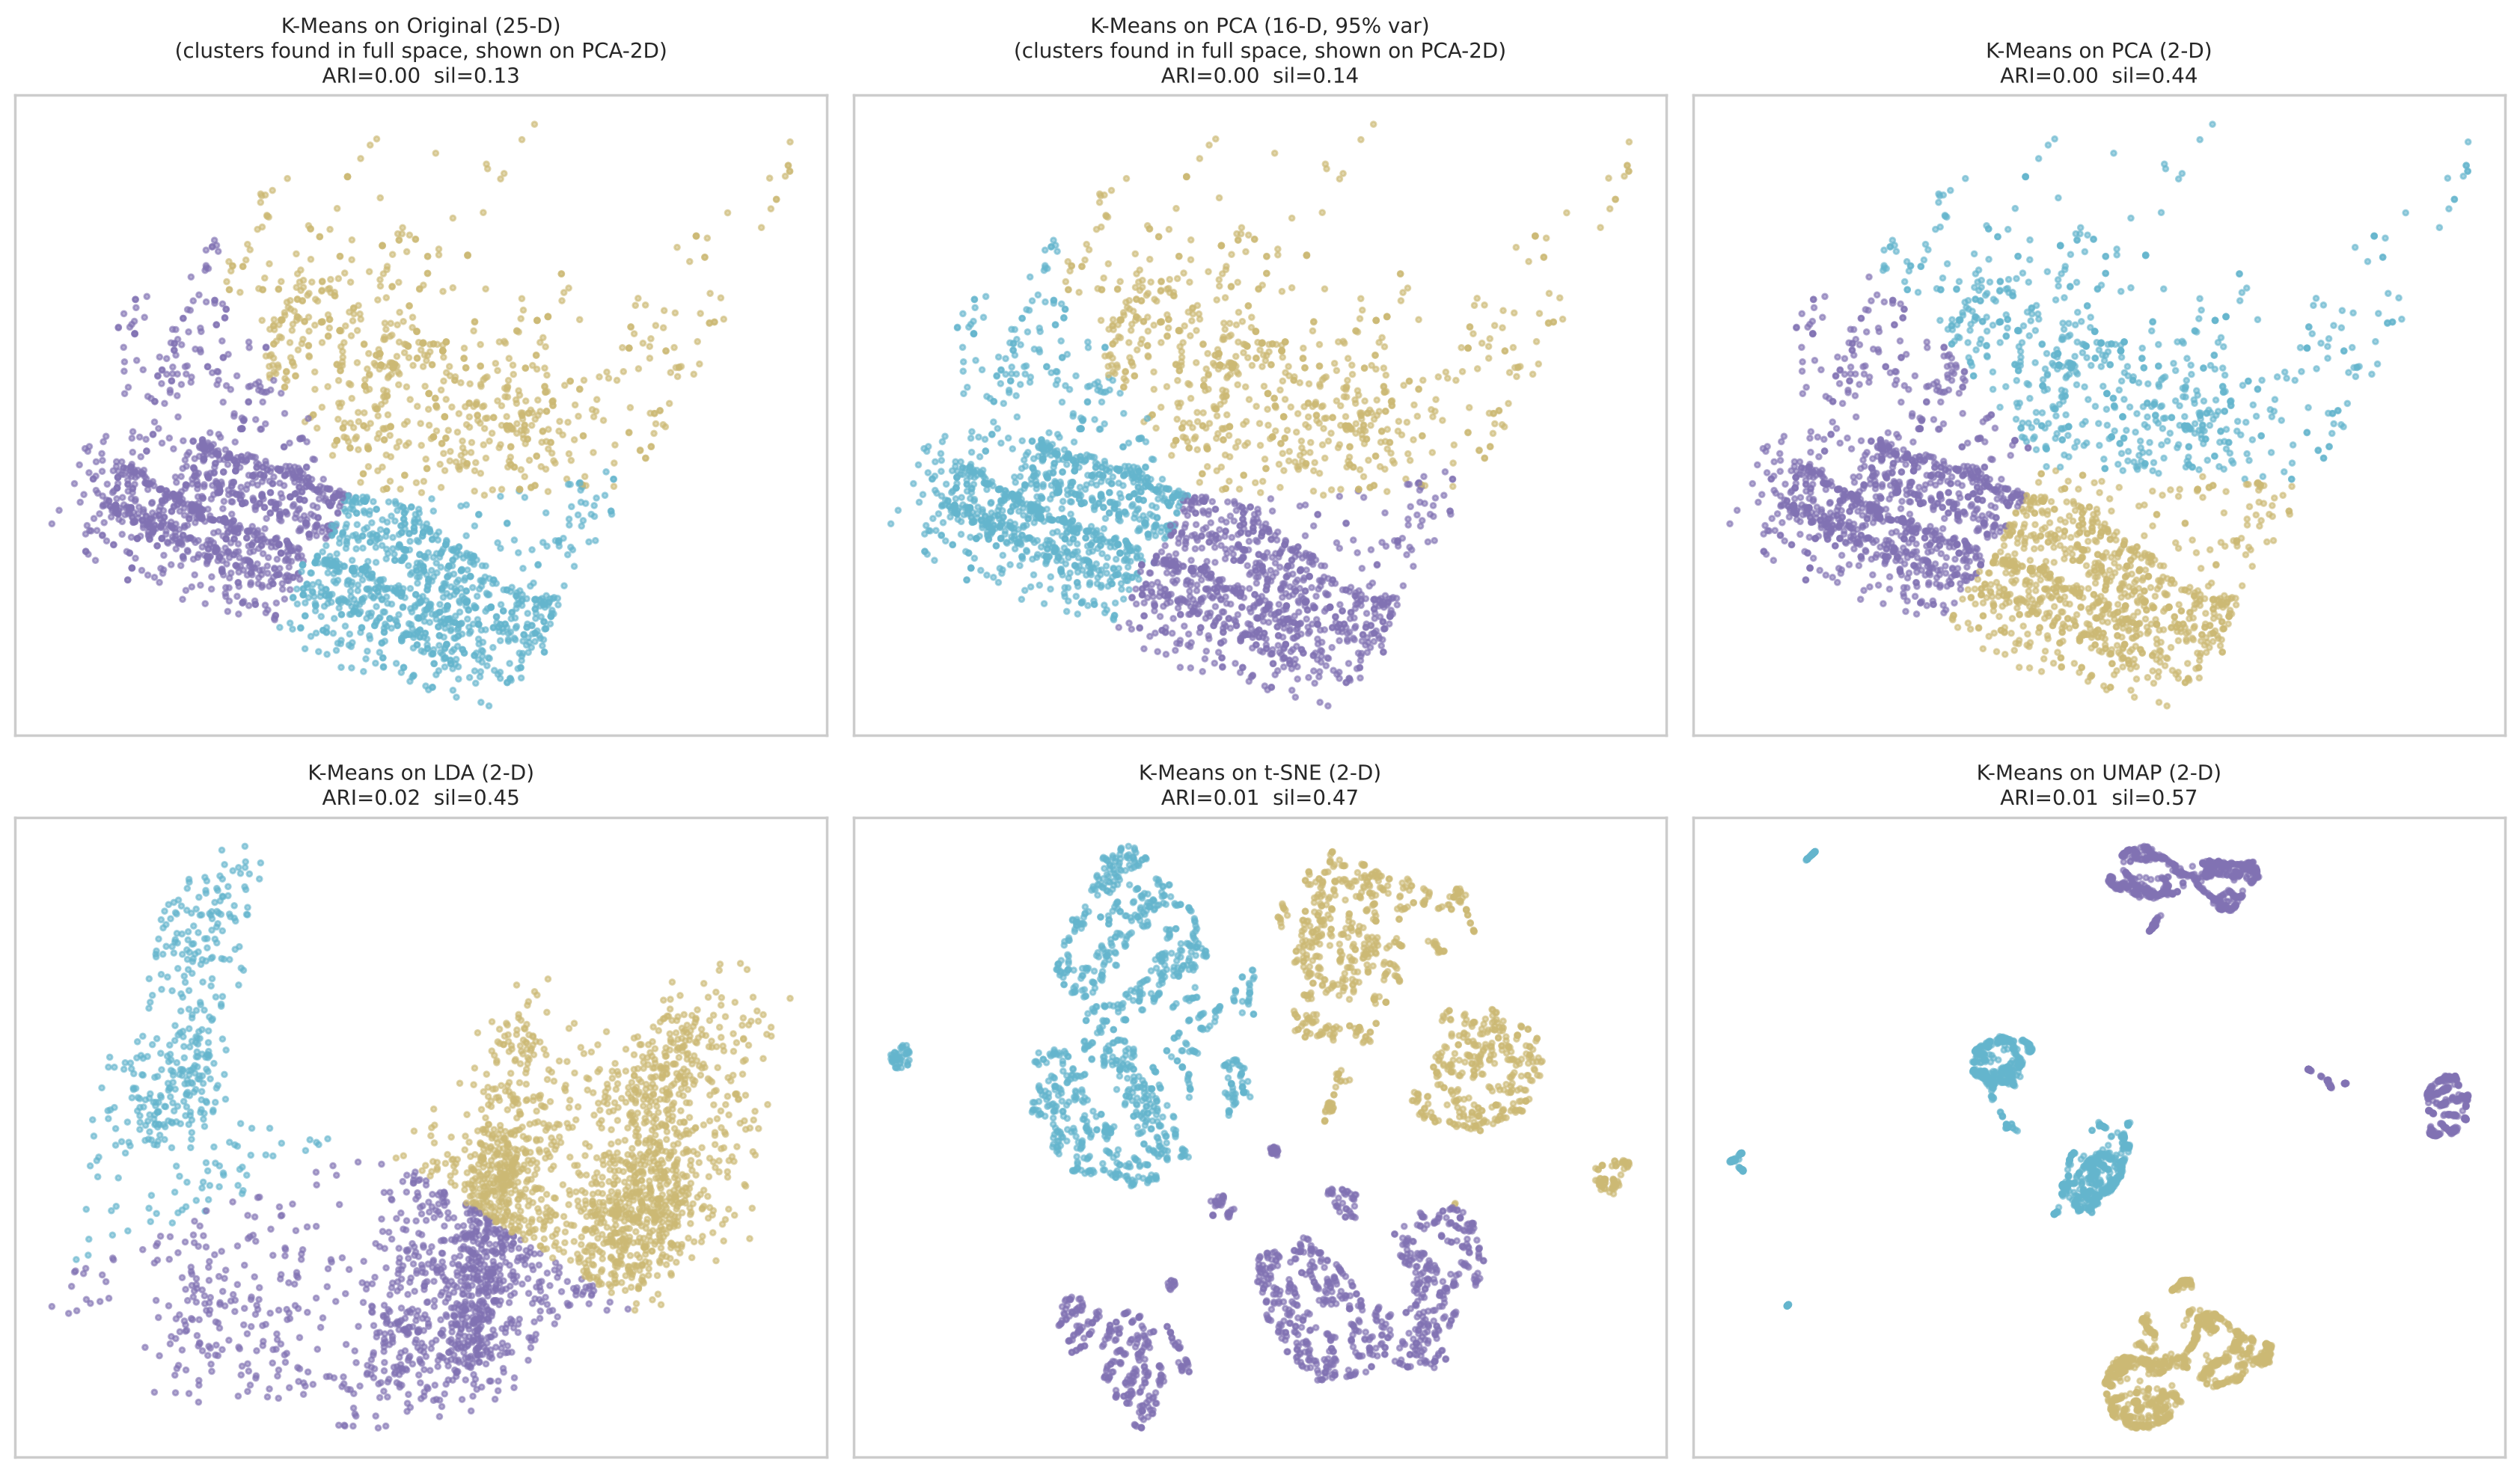
\includegraphics[width=0.92\textwidth]{figures/07_clustering_before_after.png}
\caption{K-Means clusters before (top-left, top-middle: found in the full space and shown on the PCA plane) and after reduction. The clusters become crisper after reduction (higher silhouette) but remain unrelated to the sales classes (ARI $\approx0$).}
\label{fig:clu}
\end{figure*}

\subsection{Filter feature selection}
Table~\ref{tab:filter} lists the ten best features by rank fusion and Fig.~\ref{fig:filter} shows three of the individual scores. The filters disagree in an instructive way. The linear and monotone statistics (Spearman, ANOVA-F, $\chi^2$) all rank \texttt{Size} and the store-type dummies at the top and give \texttt{Dept} only a modest score ($|\rho|=0.027$). Mutual information, which captures arbitrary dependence, ranks \texttt{Dept} first by a wide margin (MI $=0.418$ nats, almost seven times the next feature, \texttt{Store} with 0.063). Rank fusion produces a compromise that keeps \texttt{Dept} (fourth) but also keeps all three redundant type dummies, three MarkDowns and \texttt{CPI}. The variance filter flags only \texttt{MarkDown3} as near-constant (min--max variance $<0.01$), because most of its mass sits at zero after imputation. Filters are fast (under one second) but blind to redundancy and interactions --- the main reason why the filter subset is the weakest of all selected subsets in Section~\ref{sec:res:subsets}.

\begin{table}[!t]
\caption{Filter scores of the ten best features by mean rank (20k training rows)}
\label{tab:filter}
\centering
\setlength{\tabcolsep}{3pt}
\begin{tabular}{lrrrrr}
\toprule
Feature & $|\rho_S|$ & ANOVA $F$ & $\chi^2$ & MI & Rank \\
\midrule
Size & 0.270 & 900.8 & 325.3 & 0.061 & 2.00 \\
Type\_A & 0.191 & 376.6 & 354.0 & 0.018 & 3.00 \\
Type\_C & 0.148 & 317.4 & 553.1 & 0.014 & 3.75 \\
Dept & 0.027 & 82.0 & 35.6 & \textbf{0.418} & 4.75 \\
Store & 0.077 & 79.9 & 28.0 & 0.063 & 4.75 \\
Type\_B & 0.104 & 147.3 & 178.1 & 0.007 & 6.50 \\
MarkDown1 & 0.027 & 38.8 & 24.5 & 0.015 & 7.50 \\
MarkDown4 & 0.050 & 27.6 & 19.0 & 0.011 & 8.25 \\
MarkDown5 & 0.025 & 27.3 & 15.0 & 0.014 & 9.25 \\
CPI & 0.025 & 10.9 & 7.3 & 0.012 & 10.50 \\
\bottomrule
\end{tabular}
\end{table}

\begin{figure*}[!t]
\centering
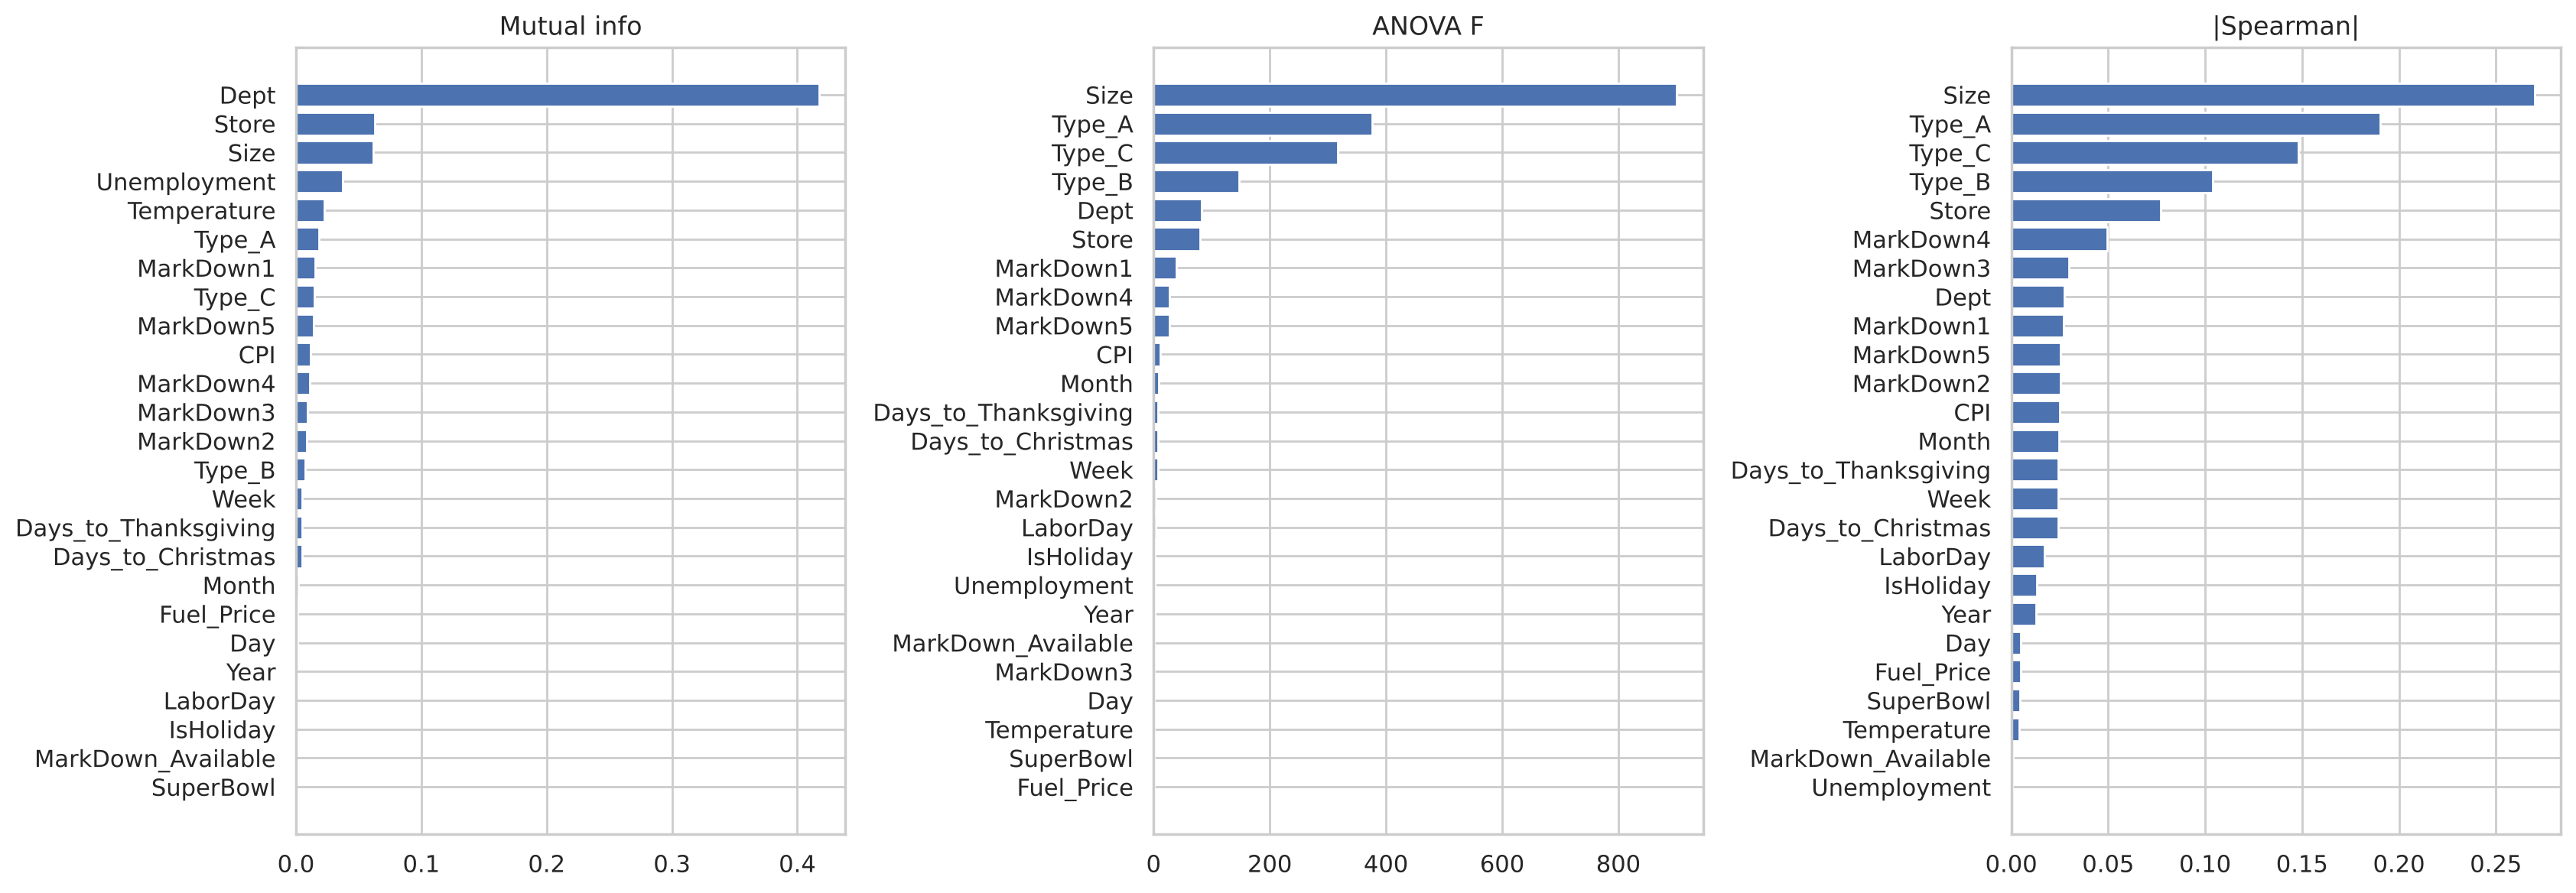
\includegraphics[width=0.95\textwidth]{figures/08_filter_scores.png}
\caption{Filter scores. Mutual information (left) is the only filter that recognises \texttt{Dept} as the dominant feature; ANOVA-F and Spearman (middle, right) favour \texttt{Size} and the store type.}
\label{fig:filter}
\end{figure*}

\subsection{Wrapper feature selection}
Each wrapper evaluates hundreds of candidate subsets with the actual learning algorithm and therefore captures interactions. All three wrappers keep the store-identity block \{\texttt{Store}, \texttt{Dept}, \texttt{Size}\} and \texttt{Week}, and they reach similar 3-fold macro-F1 on the selection sample: SFS-forward 0.871, SFS-backward 0.867 and RFE 0.866. They differ in what they add. Forward selection adds the cheap categorical context (store type, holiday flags), backward selection keeps three MarkDowns plus \texttt{CPI} and \texttt{Unemployment}, and RFE --- driven by random-forest impurity importance, which is biased towards high-cardinality continuous variables --- keeps the four economic variables and two calendar variables. Their costs differ widely: RFE took 14\,s, SFS-forward 99\,s and SFS-backward 201\,s, because backward elimination must evaluate large subsets in its first steps.

\subsection{Embedded feature selection}
The regularised logistic regressions show how much the penalty shapes the selection (Fig.~\ref{fig:emb}). With $C=0.05$, L1 sets 6 of 25 coefficient vectors to exactly zero (19 kept), Elastic-Net sets 4 to zero (21 kept), and L2, as expected, sets none to zero, so its ten largest coefficient norms are used. All three models agree on the ordering of the top features --- \texttt{Size}, \texttt{Type\_C}, \texttt{Dept}, \texttt{Type\_B}, \texttt{CPI} --- and all three reach only 44.1\% accuracy even on the data they were fitted on. This is the clearest evidence of \emph{under-fitting} in the study. A linear model cannot represent the effect of a nominal identifier such as \texttt{Dept}, so the penalty is selecting among features of a model that is itself inadequate, and the selected subsets inherit that limitation (Section~\ref{sec:res:subsets}). The gain importance of LightGBM, a non-linear embedded selector, paints a very different picture: \texttt{Dept} alone accounts for \textbf{67.0\%} of the total gain, \texttt{Size} for 14.5\% and \texttt{Store} for 4.8\%, while the 15 weakest features together contribute less than 4\%.

\begin{figure*}[!t]
\centering
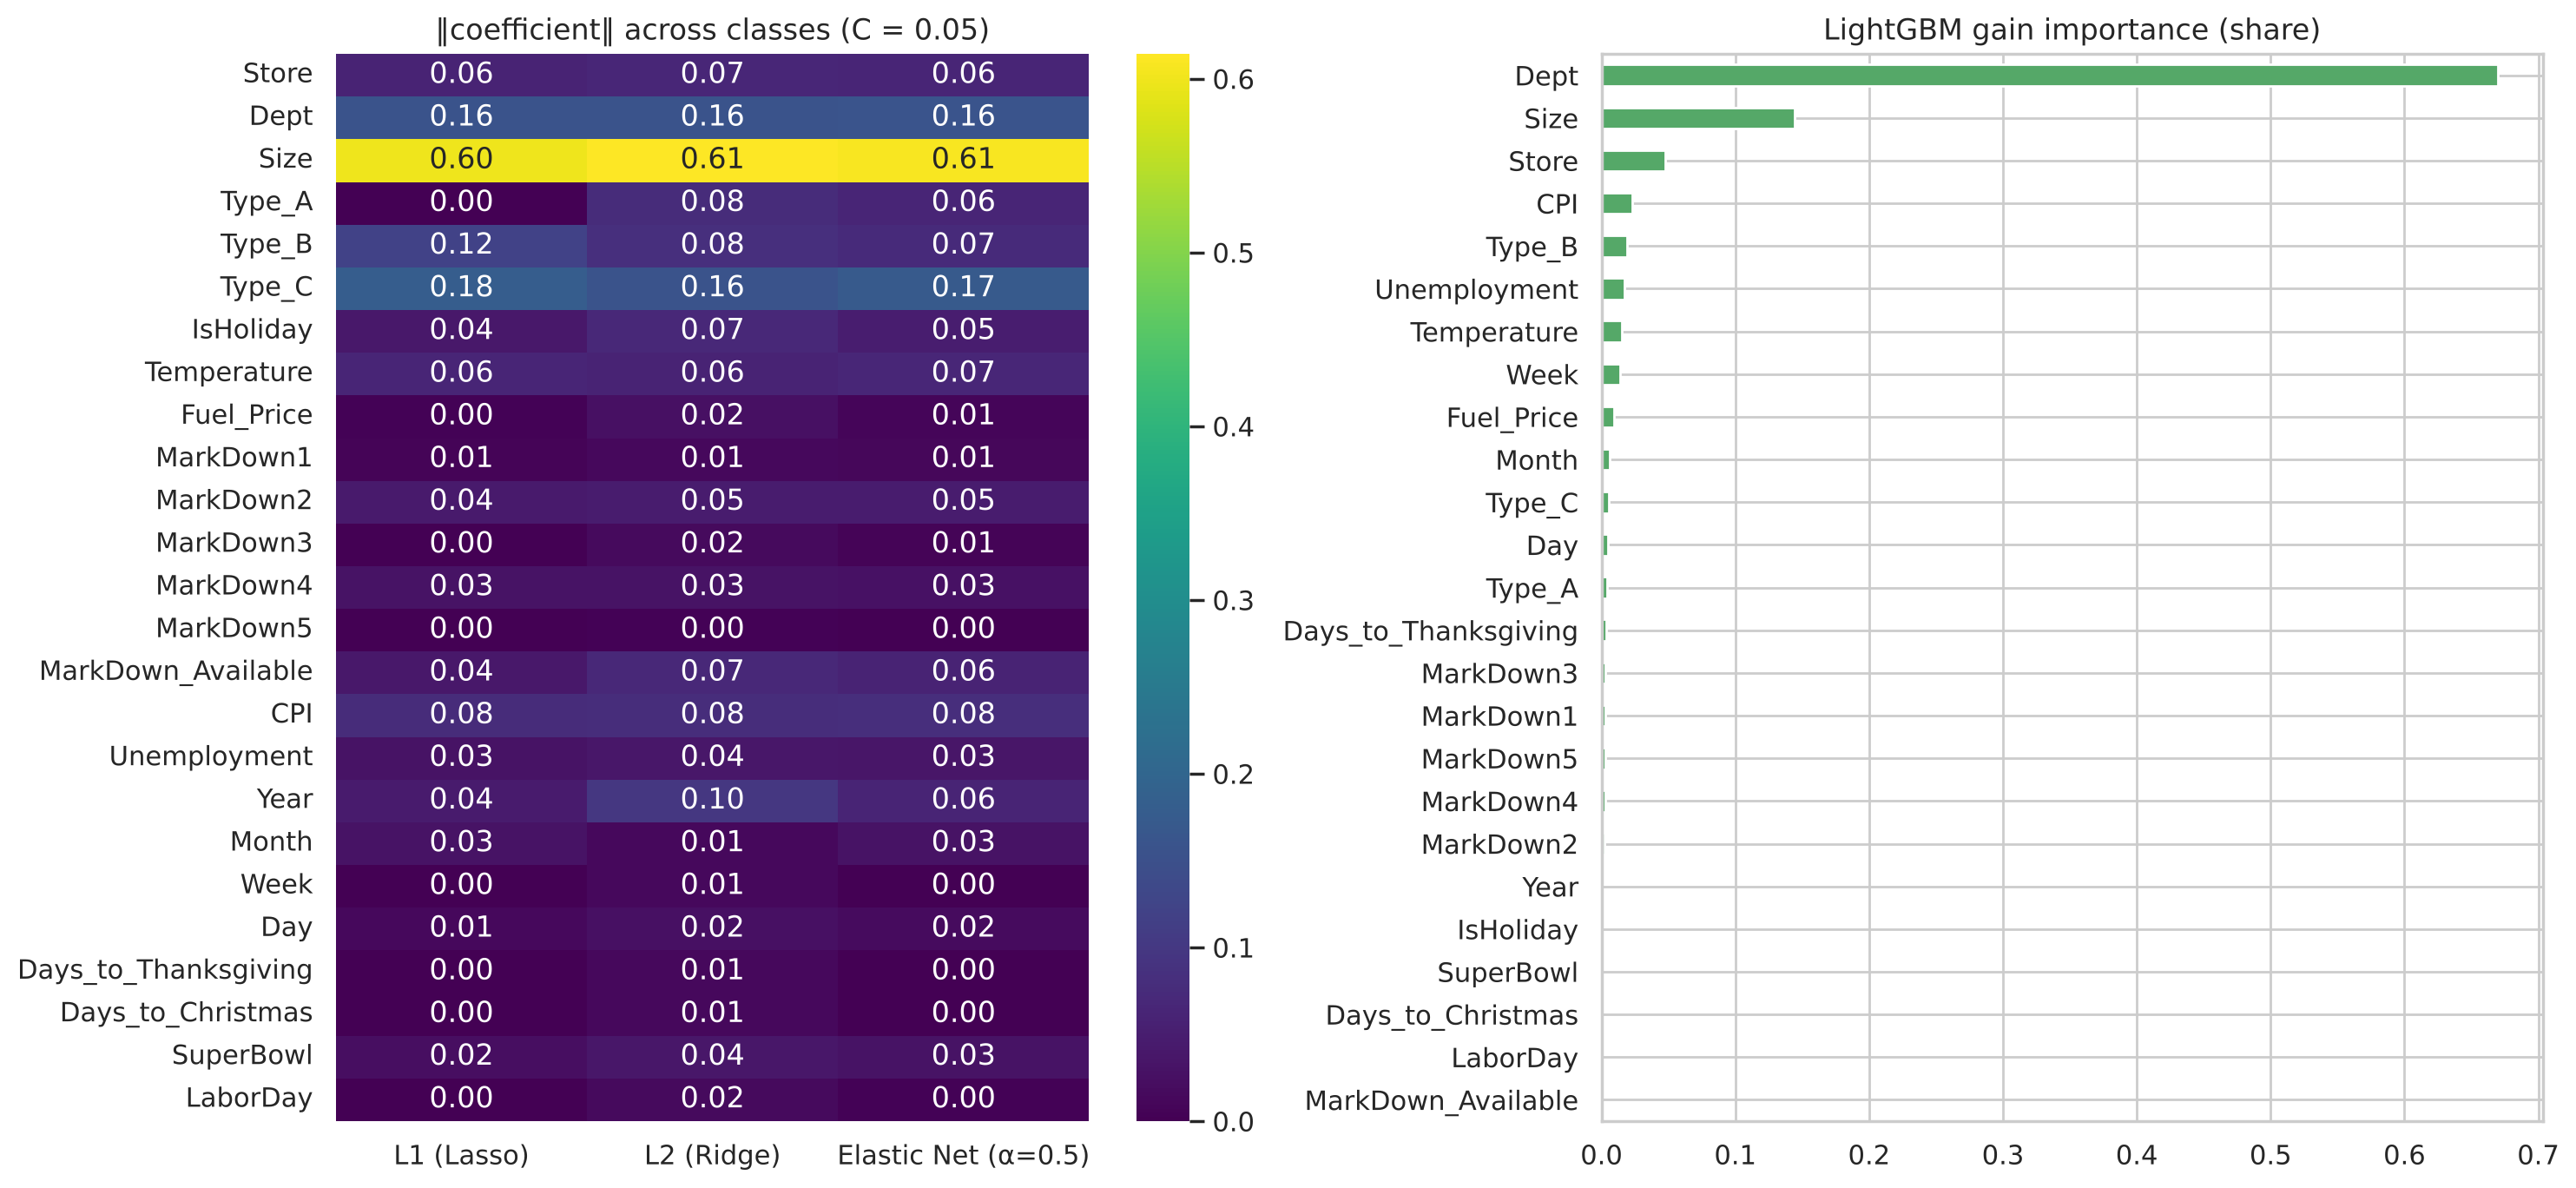
\includegraphics[width=0.9\textwidth]{figures/09_embedded.png}
\caption{Embedded selection. Left: norm of the multinomial logistic-regression coefficients under L1, L2 and Elastic-Net penalties (zero = removed). Right: LightGBM gain share, dominated by \texttt{Dept}.}
\label{fig:emb}
\end{figure*}

\subsection{Metaheuristic feature selection}
Table~\ref{tab:meta} and Fig.~\ref{fig:meta} summarise the three metaheuristics, which all optimise the size-penalised fitness of Eq.~(\ref{eq:fitness}). All three converge to very similar regions of the search space and keep the same core \{\texttt{Store}, \texttt{Dept}, \texttt{Size}, \texttt{Type\_B}\}, which is a strong sign that this core is genuinely sufficient. The GA keeps \textbf{6 features} (core + \texttt{CPI} + \texttt{Week}). BPSO keeps 9 (core + \texttt{CPI}, \texttt{IsHoliday} and three holiday-distance variables). SA keeps only \textbf{5} (core + \texttt{Days\_to\_Thanksgiving}). On the selection sample SA attains the best fitness (0.869) and F1 (0.873), followed by the GA (0.867 / 0.872) and BPSO (0.863 / 0.870). The differences are within the noise of a 3-fold estimate.

The convergence curves (Fig.~\ref{fig:meta}) show the typical behaviour of the three algorithms. The GA improves in a few large jumps during its first generations, when crossover recombines good building blocks, and then stabilises. BPSO improves steadily as the swarm contracts around the global best. SA starts from a random mask and climbs slowly, with occasional accepted downhill moves while the temperature is high. Thanks to fitness caching, the numbers of unique subsets actually evaluated were 331 (GA), 400 (BPSO) and 248 (SA), costing 193\,s, 242\,s and 151\,s. That is roughly the cost of backward SFS, but the search yields subsets two to four times smaller.

\begin{table}[!t]
\caption{Metaheuristic feature selection (fitness of Eq.~(\ref{eq:fitness}), $\lambda=0.02$; 3-fold macro-F1 on 20k training rows)}
\label{tab:meta}
\centering
\setlength{\tabcolsep}{3.5pt}
\begin{tabular}{lccccr}
\toprule
Algorithm & \#feat. & F1 & Fitness & Evals & Time (s) \\
\midrule
GA & 6 & 0.872 & 0.867 & 331 & 193 \\
Binary PSO & 9 & 0.870 & 0.863 & 400 & 242 \\
Simulated Annealing & \textbf{5} & \textbf{0.873} & \textbf{0.869} & 248 & 151 \\
\bottomrule
\end{tabular}
\vspace{2pt}
\begin{tabular}{p{8.1cm}}
\footnotesize GA: Store, Dept, Size, Type\_B, CPI, Week.\; BPSO: Store, Dept, Size, Type\_B, IsHoliday, CPI, Days\_to\_Thanksgiving, SuperBowl, LaborDay.\; SA: Store, Dept, Size, Type\_B, Days\_to\_Thanksgiving.
\end{tabular}
\end{table}

\begin{figure}[!t]
\centering
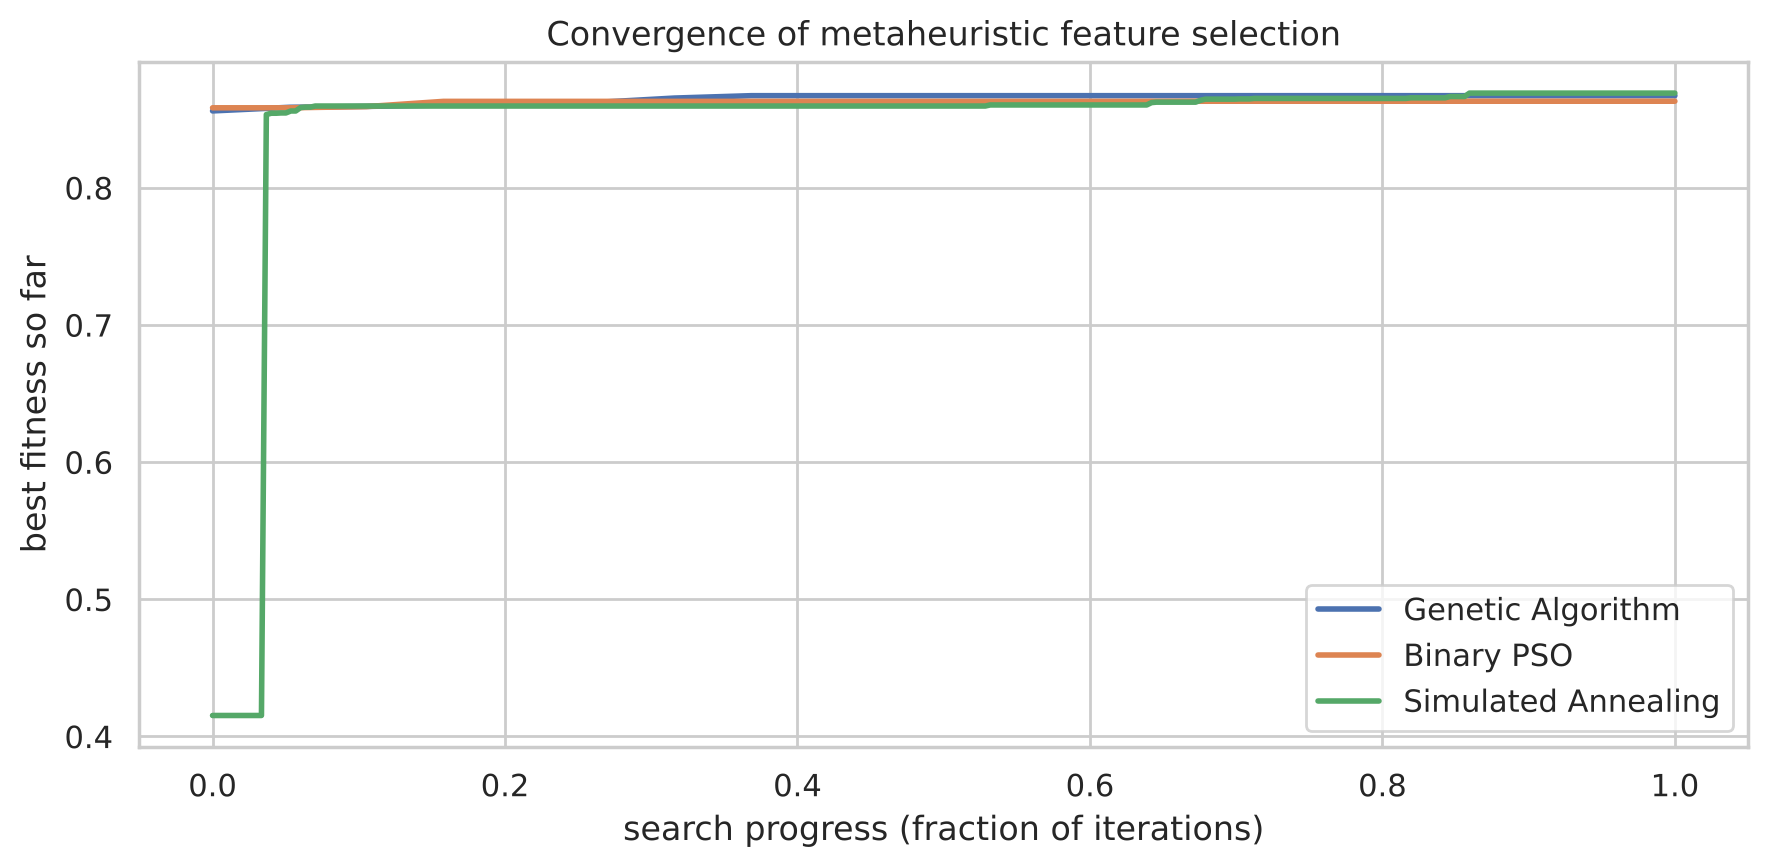
\includegraphics[width=\columnwidth]{figures/10_metaheuristic_convergence.png}
\caption{Convergence of the best fitness for GA, BPSO and SA (x-axis normalised to the fraction of iterations).}
\label{fig:meta}
\end{figure}

\subsection{Consensus across selection methods}
Fig.~\ref{fig:freq} counts how often each feature is chosen by the eleven selectors. \texttt{Store}, \texttt{Dept} and \texttt{Size} are chosen by all eleven, \texttt{Type\_B} by ten and \texttt{CPI} by nine. At the other end, \texttt{Days\_to\_Christmas} is never chosen --- it is a perfect linear copy of \texttt{Days\_to\_Thanksgiving} within each year --- and \texttt{MarkDown3} and \texttt{MarkDown5} are each chosen twice. This consensus provides a robust, method-independent answer to the question ``which variables matter'': the \emph{identity and size of the store-department} first, the macro-economic context a distant second, and the promotions and holiday flags hardly at all once the identity is known.

\begin{figure}[!t]
\centering
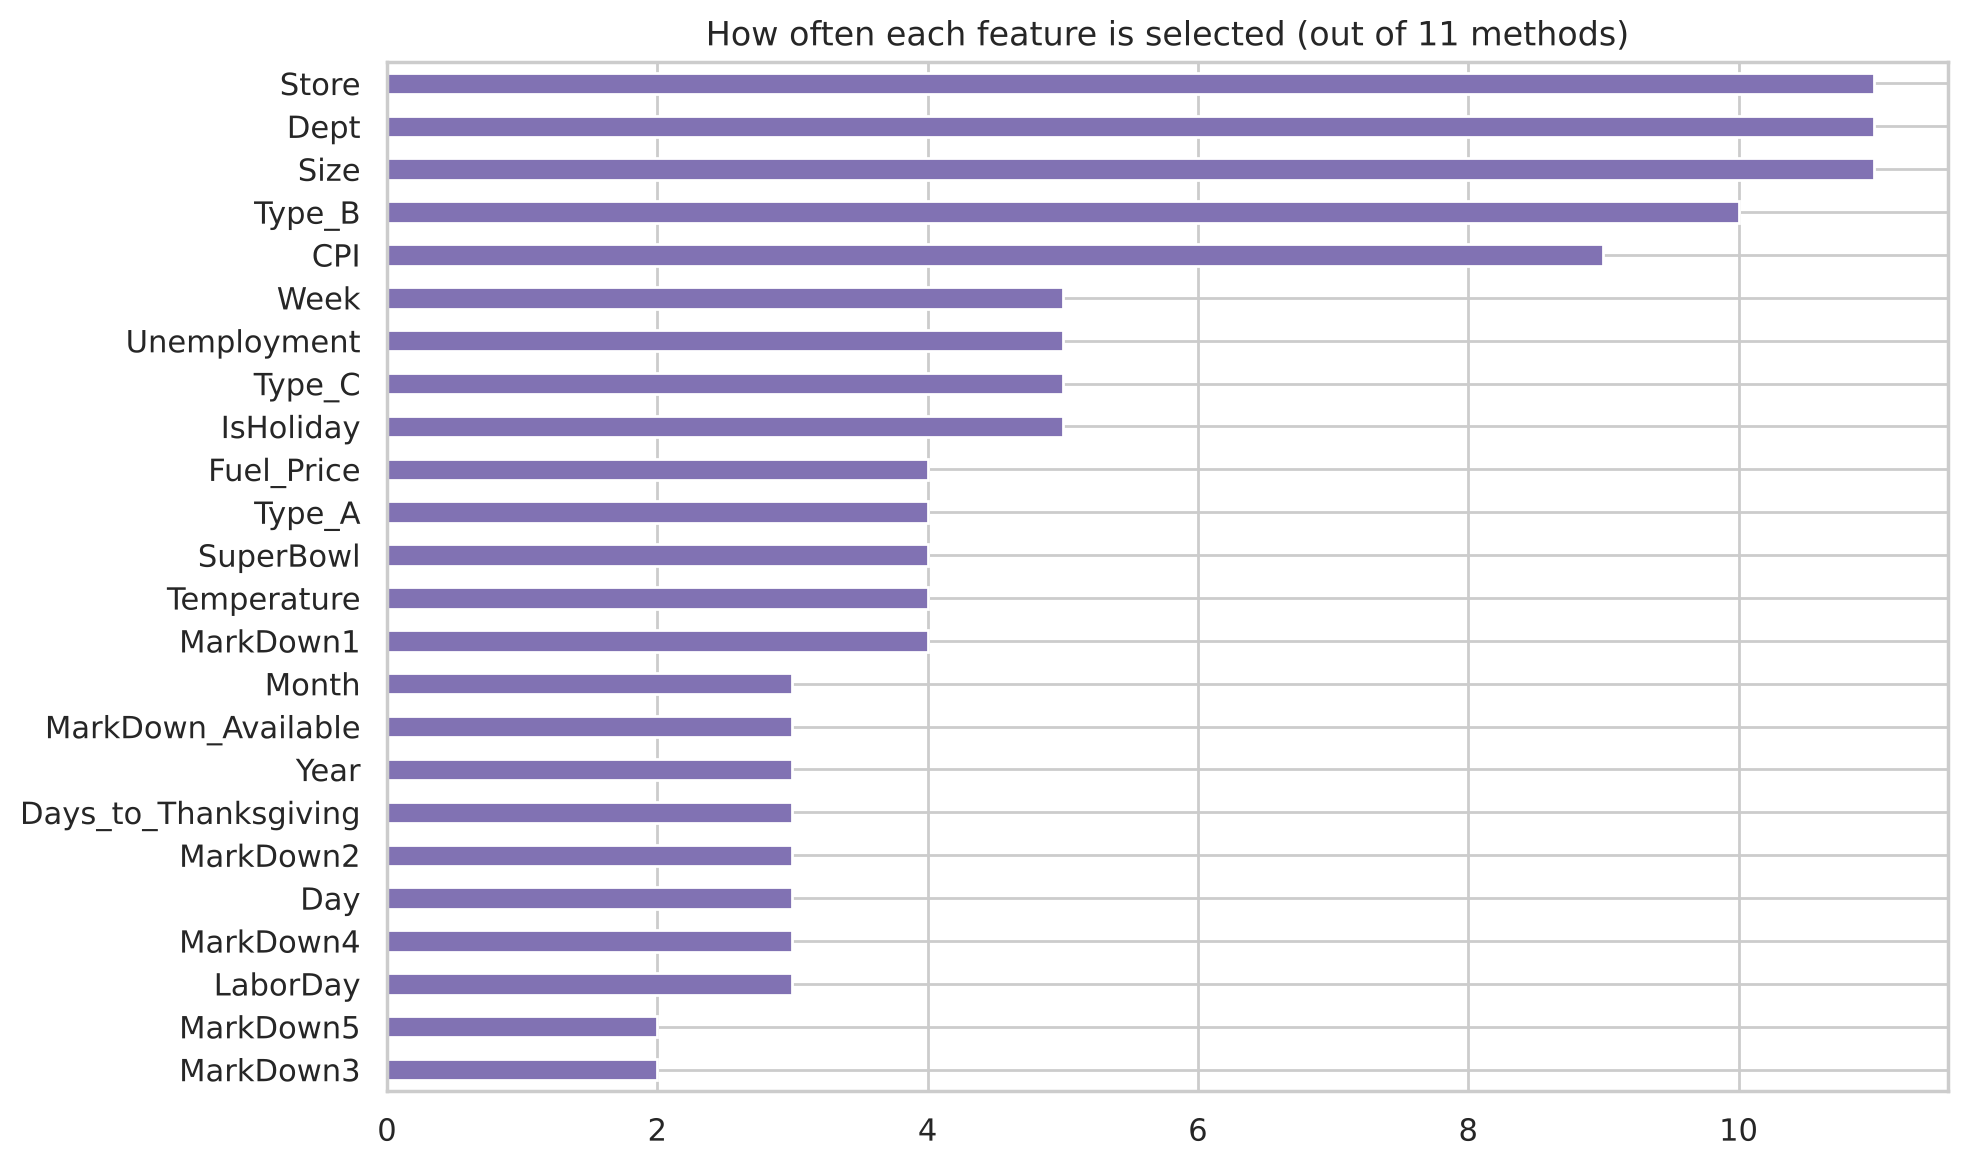
\includegraphics[width=\columnwidth]{figures/11_selection_frequency.png}
\caption{Selection frequency of each feature across the eleven selection methods.}
\label{fig:freq}
\end{figure}

\subsection{Selection before reduction}\label{sec:res:ras}
The negative result for the embeddings raises a natural question: is the weak class structure intrinsic, or is it caused by the noisy context variables, which dominate Euclidean distances? To answer it we repeated PCA, LDA, t-SNE and UMAP on the same 3{,}000 points using only the six GA-selected features (Table~\ref{tab:ras}, Fig.~\ref{fig:ras}). The effect is large for the unsupervised methods. The 5-NN accuracy rises from 37.1\% to \textbf{50.5\%} for PCA (+13.4 points), from 39.5\% to \textbf{51.5\%} for t-SNE (+12.0) and from 38.8\% to \textbf{50.0\%} for UMAP (+11.2), and trustworthiness also improves (t-SNE 0.999, UMAP 0.998, PCA 0.938). LDA is unchanged (46.3\% $\to$ 46.1\%) because, being supervised, it already down-weights irrelevant directions. K-Means still does not recover the classes (ARI $\le0.03$). Even with clean inputs, the sales level depends on department identity in a way that no compact geometric cluster captures.

The practical lesson is that \emph{feature selection should precede feature reduction} when the goal is a class-aware low-dimensional view of noisy tabular data. Unsupervised reduction treats every input dimension as equally important and cannot tell signal from noise on its own.

\begin{table}[!t]
\caption{Reduction after GA selection: 5-NN accuracy and trustworthiness on all 25 features vs.\ the 6 GA features}
\label{tab:ras}
\centering
\begin{tabular}{lcccc}
\toprule
 & \multicolumn{2}{c}{kNN accuracy} & & \\
\cmidrule{2-3}
Method & All 25 & GA 6 & $\Delta$ & Trustw.\ (GA) \\
\midrule
PCA & 0.371 & 0.505 & $+0.134$ & 0.938 \\
LDA & 0.463 & 0.461 & $-0.002$ & 0.891 \\
t-SNE & 0.395 & \textbf{0.515} & $+0.120$ & 0.999 \\
UMAP & 0.388 & 0.500 & $+0.112$ & 0.998 \\
\bottomrule
\end{tabular}
\end{table}

\begin{figure*}[!t]
\centering
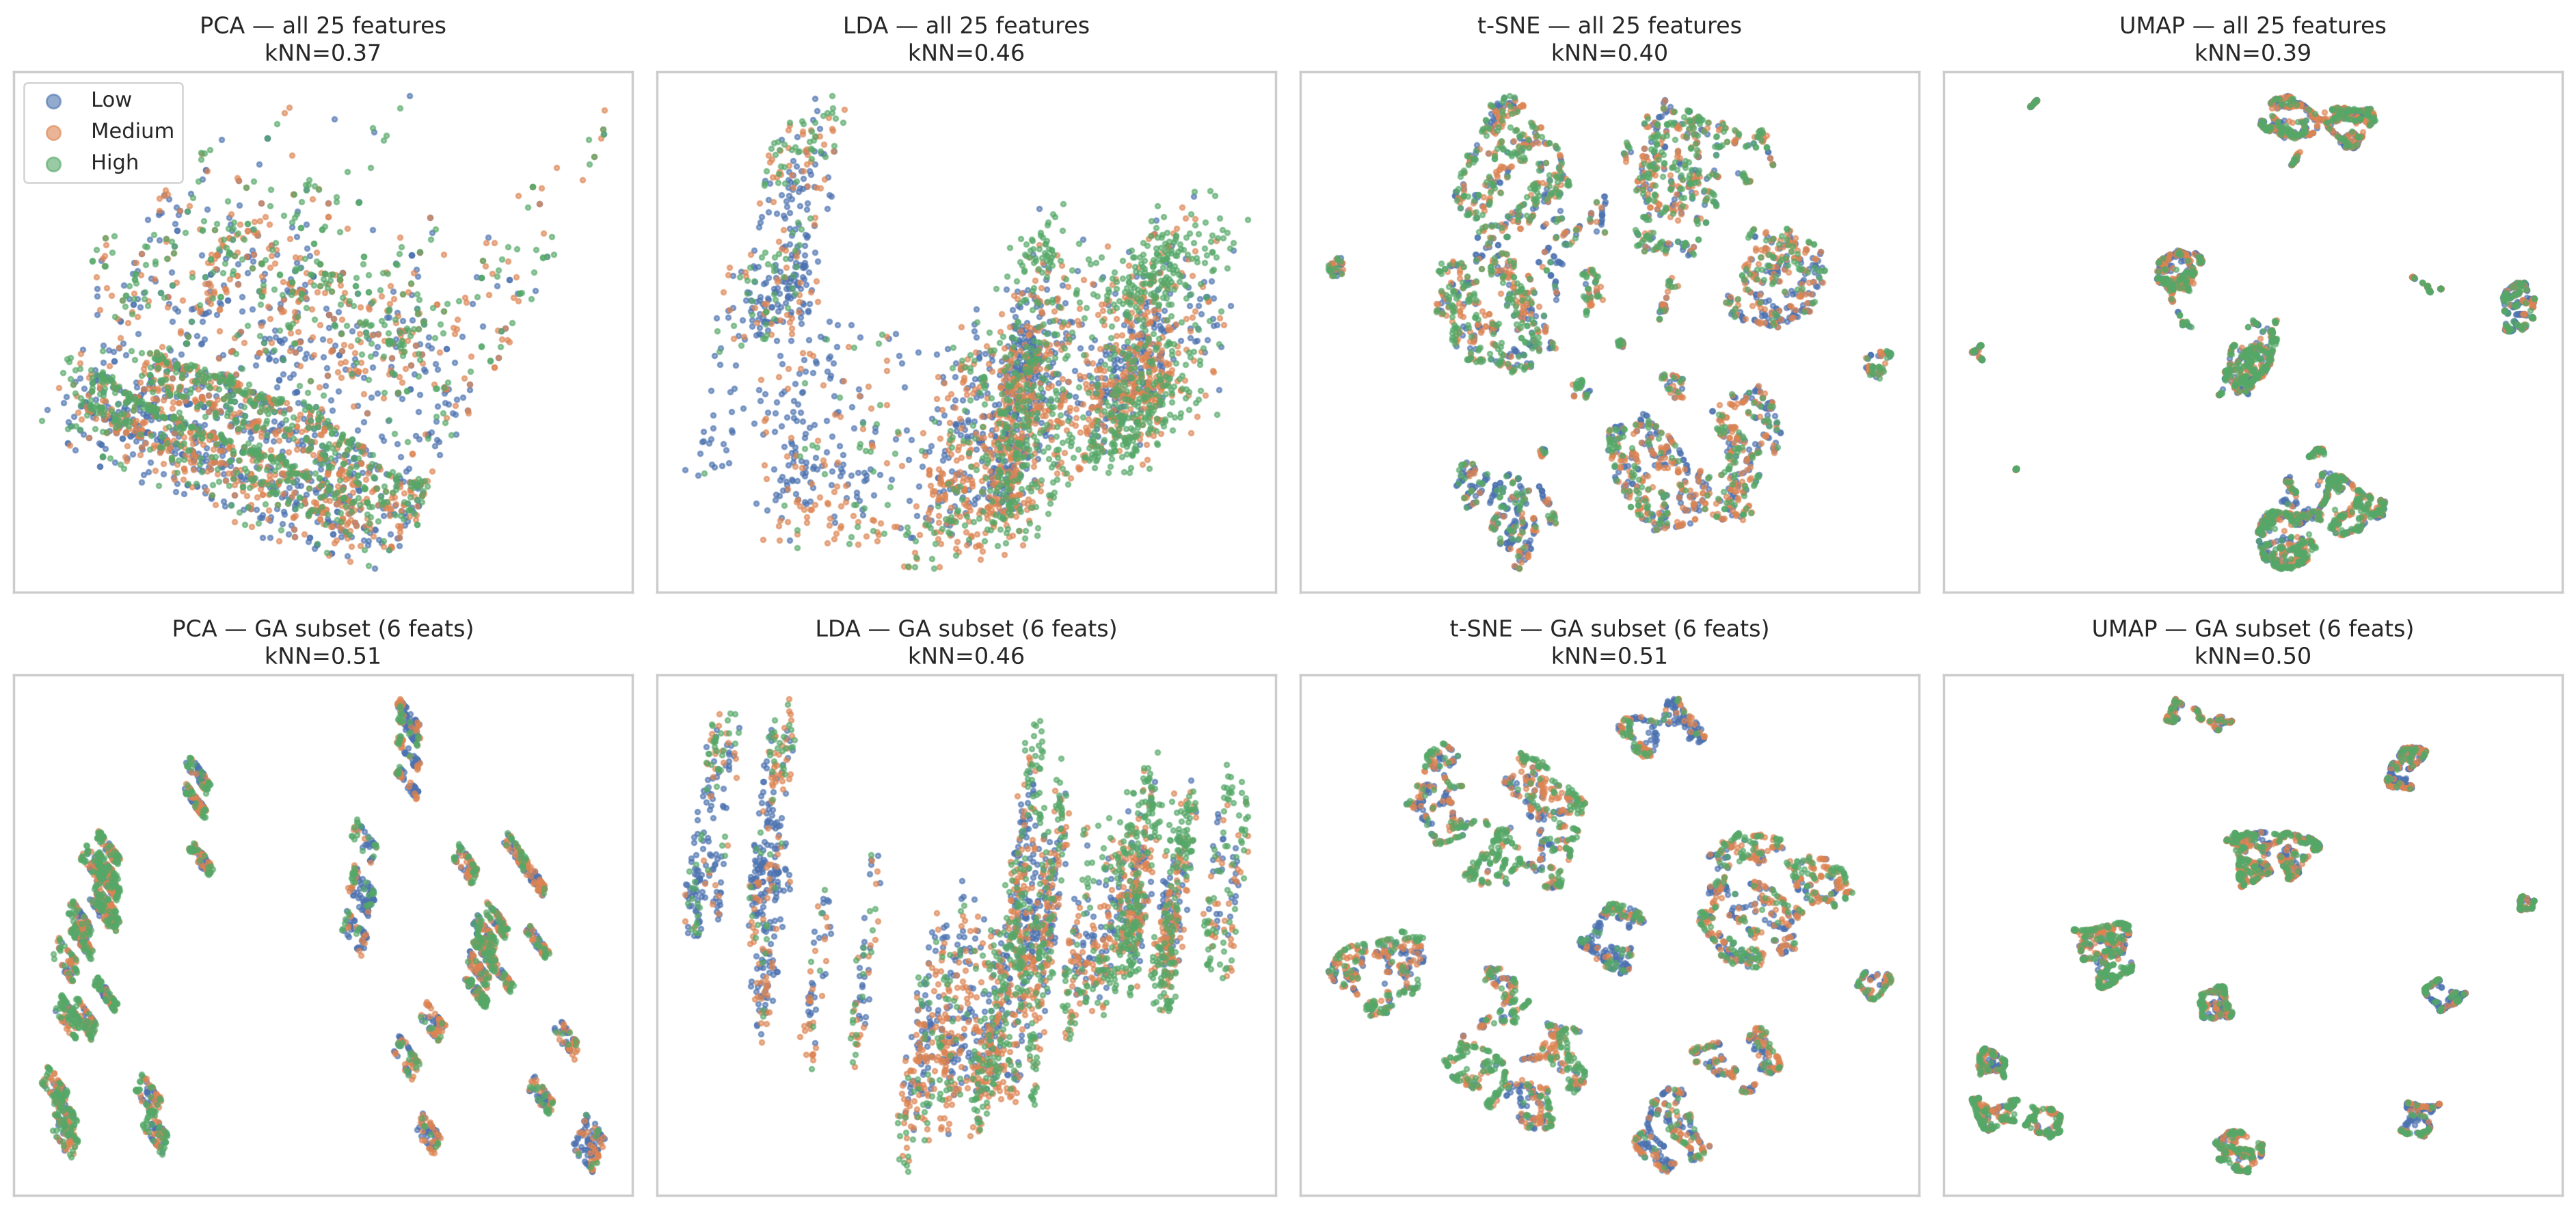
\includegraphics[width=\textwidth]{figures/17_reduction_after_selection.png}
\caption{The same 3{,}000 points embedded from all 25 features (top) and from the 6 GA-selected features (bottom). Removing noisy context variables before reduction gives markedly more class-coherent neighbourhoods.}
\label{fig:ras}
\end{figure*}

\subsection{Classification models: hold-out results}\label{sec:res:models}
Table~\ref{tab:hold} reports all requested metrics on the 20\% test split, sorted by macro-F1. Because the classes are balanced, macro precision, recall and F1 are almost equal to accuracy for every model.

The nine models fall into three clearly separated tiers. \textbf{Gradient boosting} is the best tier: LightGBM reaches \textbf{93.44\% accuracy} (error rate 6.56\%), macro-F1 0.934 and ROC-AUC 0.991, with XGBoost a close second (93.18\%, AUC 0.990). The \textbf{unpruned decision tree} forms the second tier on its own (90.18\%), but its ROC-AUC is much lower (0.926) because a fully grown tree outputs almost hard 0/1 probabilities that rank poorly. The third tier contains every model that cannot exploit \texttt{Dept} as a nominal identifier: the MLP (68.98\%), the random forest (67.08\%), extra trees (60.08\%), $k$-NN (50.80\%), Gaussian naive Bayes (46.16\%) and logistic regression (44.39\%). These are only 11--36 points above the 33.3\% chance level.

\begin{table*}[!t]
\caption{Hold-out evaluation (80{,}000 train / 20{,}000 test rows, all 25 features). Precision, recall and F1 are macro-averaged; ROC-AUC is one-vs-rest macro. Gap = train $-$ test accuracy}
\label{tab:hold}
\centering
\begin{tabular}{lcccccccccl}
\toprule
Model & Train acc. & Test acc. & Error rate & Precision & Recall & F1 & ROC-AUC & Gap & Fit (s) & Diagnosis \\
\midrule
LightGBM & 0.9929 & \textbf{0.9344} & \textbf{0.0656} & \textbf{0.9344} & \textbf{0.9344} & \textbf{0.9344} & \textbf{0.9906} & 0.059 & 9.2 & Slight over-fit \\
XGBoost & 0.9874 & 0.9318 & 0.0682 & 0.9319 & 0.9319 & 0.9318 & 0.9899 & 0.056 & 7.7 & Slight over-fit \\
Decision Tree & 1.0000 & 0.9018 & 0.0981 & 0.9018 & 0.9019 & 0.9018 & 0.9264 & 0.098 & 0.6 & Over-fitting \\
MLP & 0.7260 & 0.6898 & 0.3102 & 0.6870 & 0.6898 & 0.6870 & 0.8524 & 0.036 & 61.7 & Under-fitting \\
Random Forest & 0.9246 & 0.6708 & 0.3293 & 0.6706 & 0.6708 & 0.6701 & 0.8496 & 0.254 & 7.4 & Over-fitting \\
Extra Trees & 0.9102 & 0.6008 & 0.3992 & 0.5981 & 0.6009 & 0.5989 & 0.7883 & 0.309 & 4.9 & Over-fitting \\
KNN ($k$=15) & 0.5916 & 0.5080 & 0.4920 & 0.5065 & 0.5081 & 0.5055 & 0.6939 & 0.084 & 0.03 & Over- \& under-fit \\
Gaussian NB & 0.4560 & 0.4616 & 0.5384 & 0.4609 & 0.4617 & 0.4601 & 0.6380 & $-0.006$ & 0.06 & Under-fitting \\
Logistic Regression & 0.4412 & 0.4439 & 0.5561 & 0.4509 & 0.4439 & 0.4434 & 0.6309 & $-0.003$ & 0.2 & Under-fitting \\
\bottomrule
\end{tabular}
\end{table*}

\subsection{K-fold cross-validation}
Table~\ref{tab:cv} gives the stratified 5-fold results on the full 100k sample and Fig.~\ref{fig:cvbox} shows the fold-wise accuracies. The CV means agree with the hold-out results to within 0.2 percentage points for every model except the MLP. This confirms that the single 80/20 split is representative and that the ranking is stable. LightGBM's average accuracy is \textbf{93.42\% $\pm$ 0.20\%}, and its worst fold (93.12\%) is still better than XGBoost's mean (93.06\%). The fold-to-fold standard deviation is tiny ($\le$0.5 points) for every model except the MLP ($\pm$2.35 points). Its accuracy ranges from 63.2\% to 69.4\% depending on the fold, a sign of an unstable optimisation driven by early stopping on a small validation fraction rather than of a data effect.

\begin{table}[!t]
\caption{Stratified 5-fold cross-validation on the 100k sample (mean $\pm$ std)}
\label{tab:cv}
\centering
\setlength{\tabcolsep}{3pt}
\begin{tabular}{lccc}
\toprule
Model & Accuracy & Macro-F1 & ROC-AUC \\
\midrule
LightGBM & \textbf{0.9342}$\pm$0.0020 & \textbf{0.9343}$\pm$0.0020 & \textbf{0.9906} \\
XGBoost & 0.9306$\pm$0.0013 & 0.9307$\pm$0.0013 & 0.9898 \\
Decision Tree & 0.9042$\pm$0.0014 & 0.9042$\pm$0.0013 & 0.9282 \\
Random Forest & 0.6699$\pm$0.0019 & 0.6695$\pm$0.0018 & 0.8492 \\
MLP & 0.6645$\pm$0.0235 & 0.6606$\pm$0.0228 & 0.8361 \\
Extra Trees & 0.5953$\pm$0.0050 & 0.5936$\pm$0.0049 & 0.7855 \\
KNN ($k$=15) & 0.5091$\pm$0.0029 & 0.5070$\pm$0.0029 & 0.6915 \\
Gaussian NB & 0.4570$\pm$0.0034 & 0.4548$\pm$0.0054 & 0.6347 \\
Logistic Reg. & 0.4410$\pm$0.0007 & 0.4403$\pm$0.0006 & 0.6294 \\
\bottomrule
\end{tabular}
\end{table}

\begin{figure}[!t]
\centering
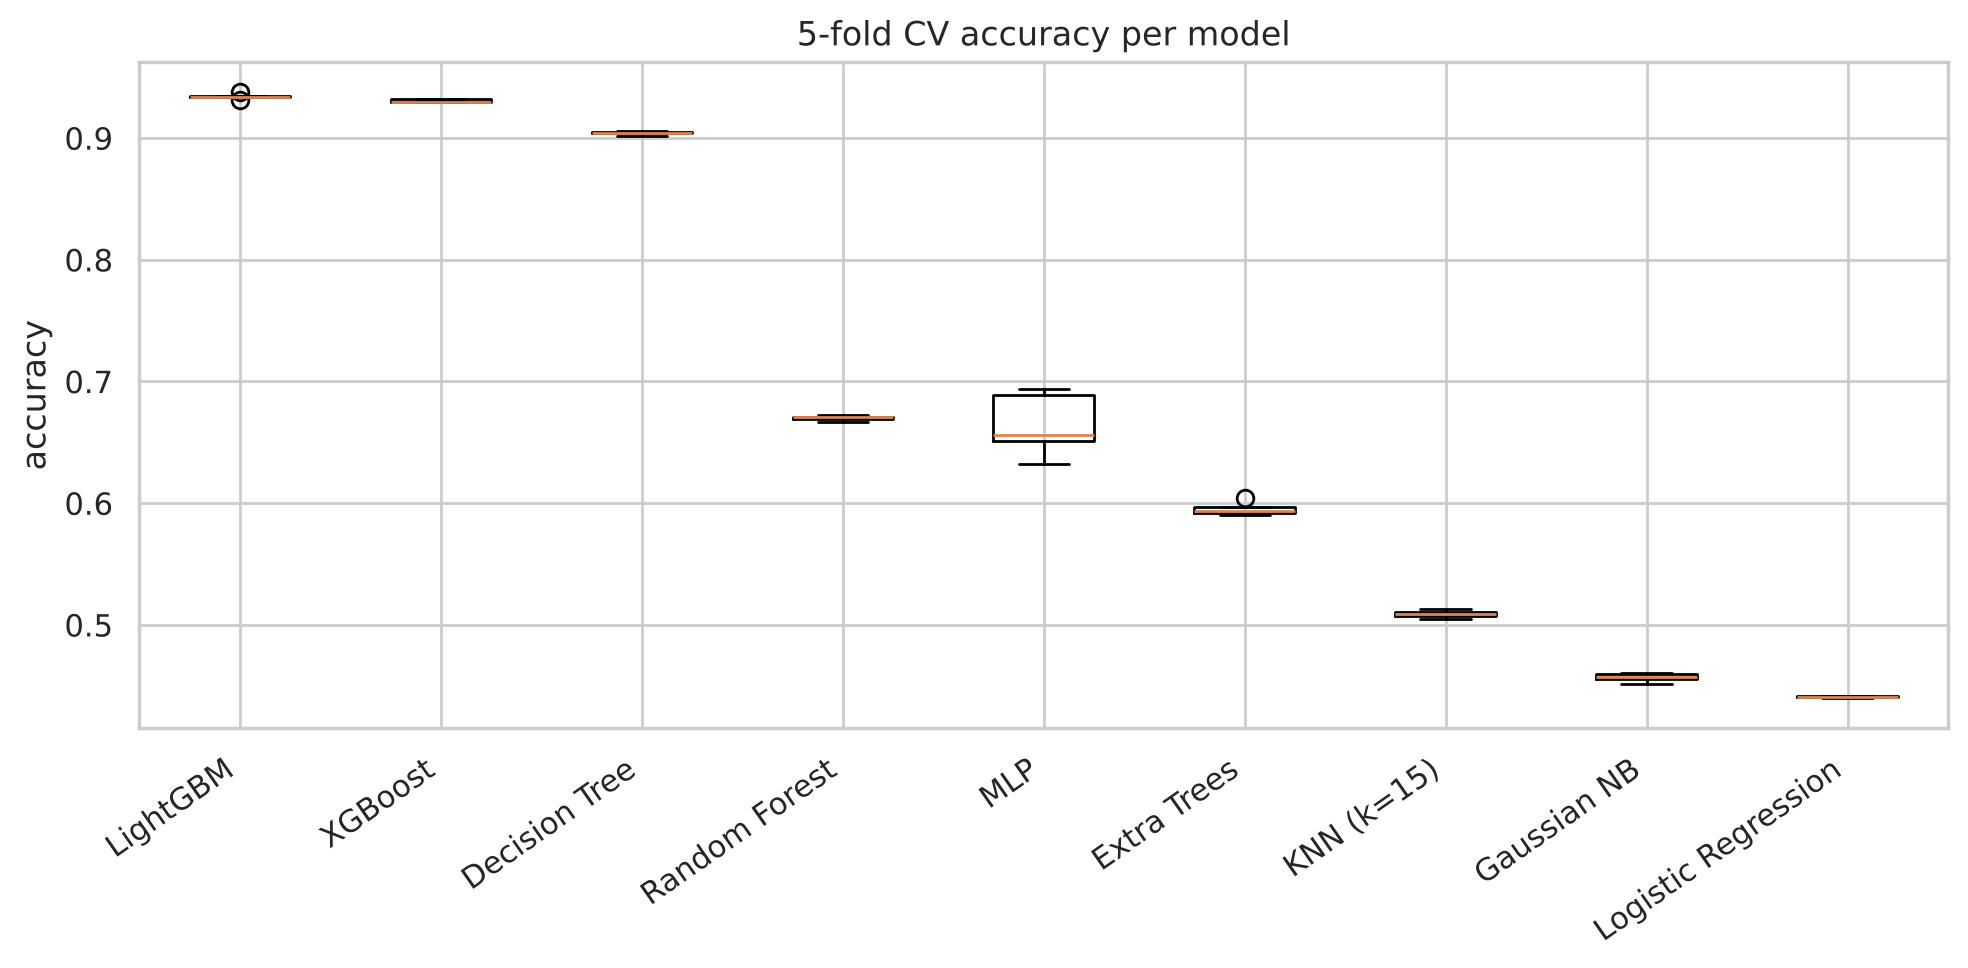
\includegraphics[width=\columnwidth]{figures/12_cv_boxplot.png}
\caption{Fold-wise 5-fold CV accuracy. Only the MLP shows a large spread.}
\label{fig:cvbox}
\end{figure}

\subsection{Confusion matrices}
Fig.~\ref{fig:cm} shows the row-normalised test confusion matrices of six models, and Table~\ref{tab:cmint} gives the per-class figures. For \textbf{LightGBM} the per-class recalls are 95.3\% (Low), 90.1\% (Medium) and 94.9\% (High). The Medium class is the hardest because it borders both other classes, while Low and High each have only one neighbour. Of LightGBM's 1{,}312 errors, the most frequent is a true Medium predicted as Low (383 cases), and only \textbf{7 errors (0.5\%) are ``far'' errors} between Low and High. The model's mistakes are therefore almost exclusively near-threshold confusions between adjacent levels, the least costly kind of error for staffing or replenishment decisions. The pattern is the same for XGBoost (9 far errors) and the decision tree (23).

For the under-fitting linear models the picture is the opposite. Logistic regression commits 11{,}122 errors, of which 3{,}094 (\textbf{27.8\%}) are far Low$\leftrightarrow$High errors, and its most common confusion is a true Medium predicted as High (2{,}698 cases). Its Medium recall is 37.2\%, barely above chance. Gaussian naive Bayes behaves similarly (26.9\% far errors). Such models do not merely blur the class boundaries; they lack any usable notion of the ordering of sales levels.

\begin{figure*}[!t]
\centering
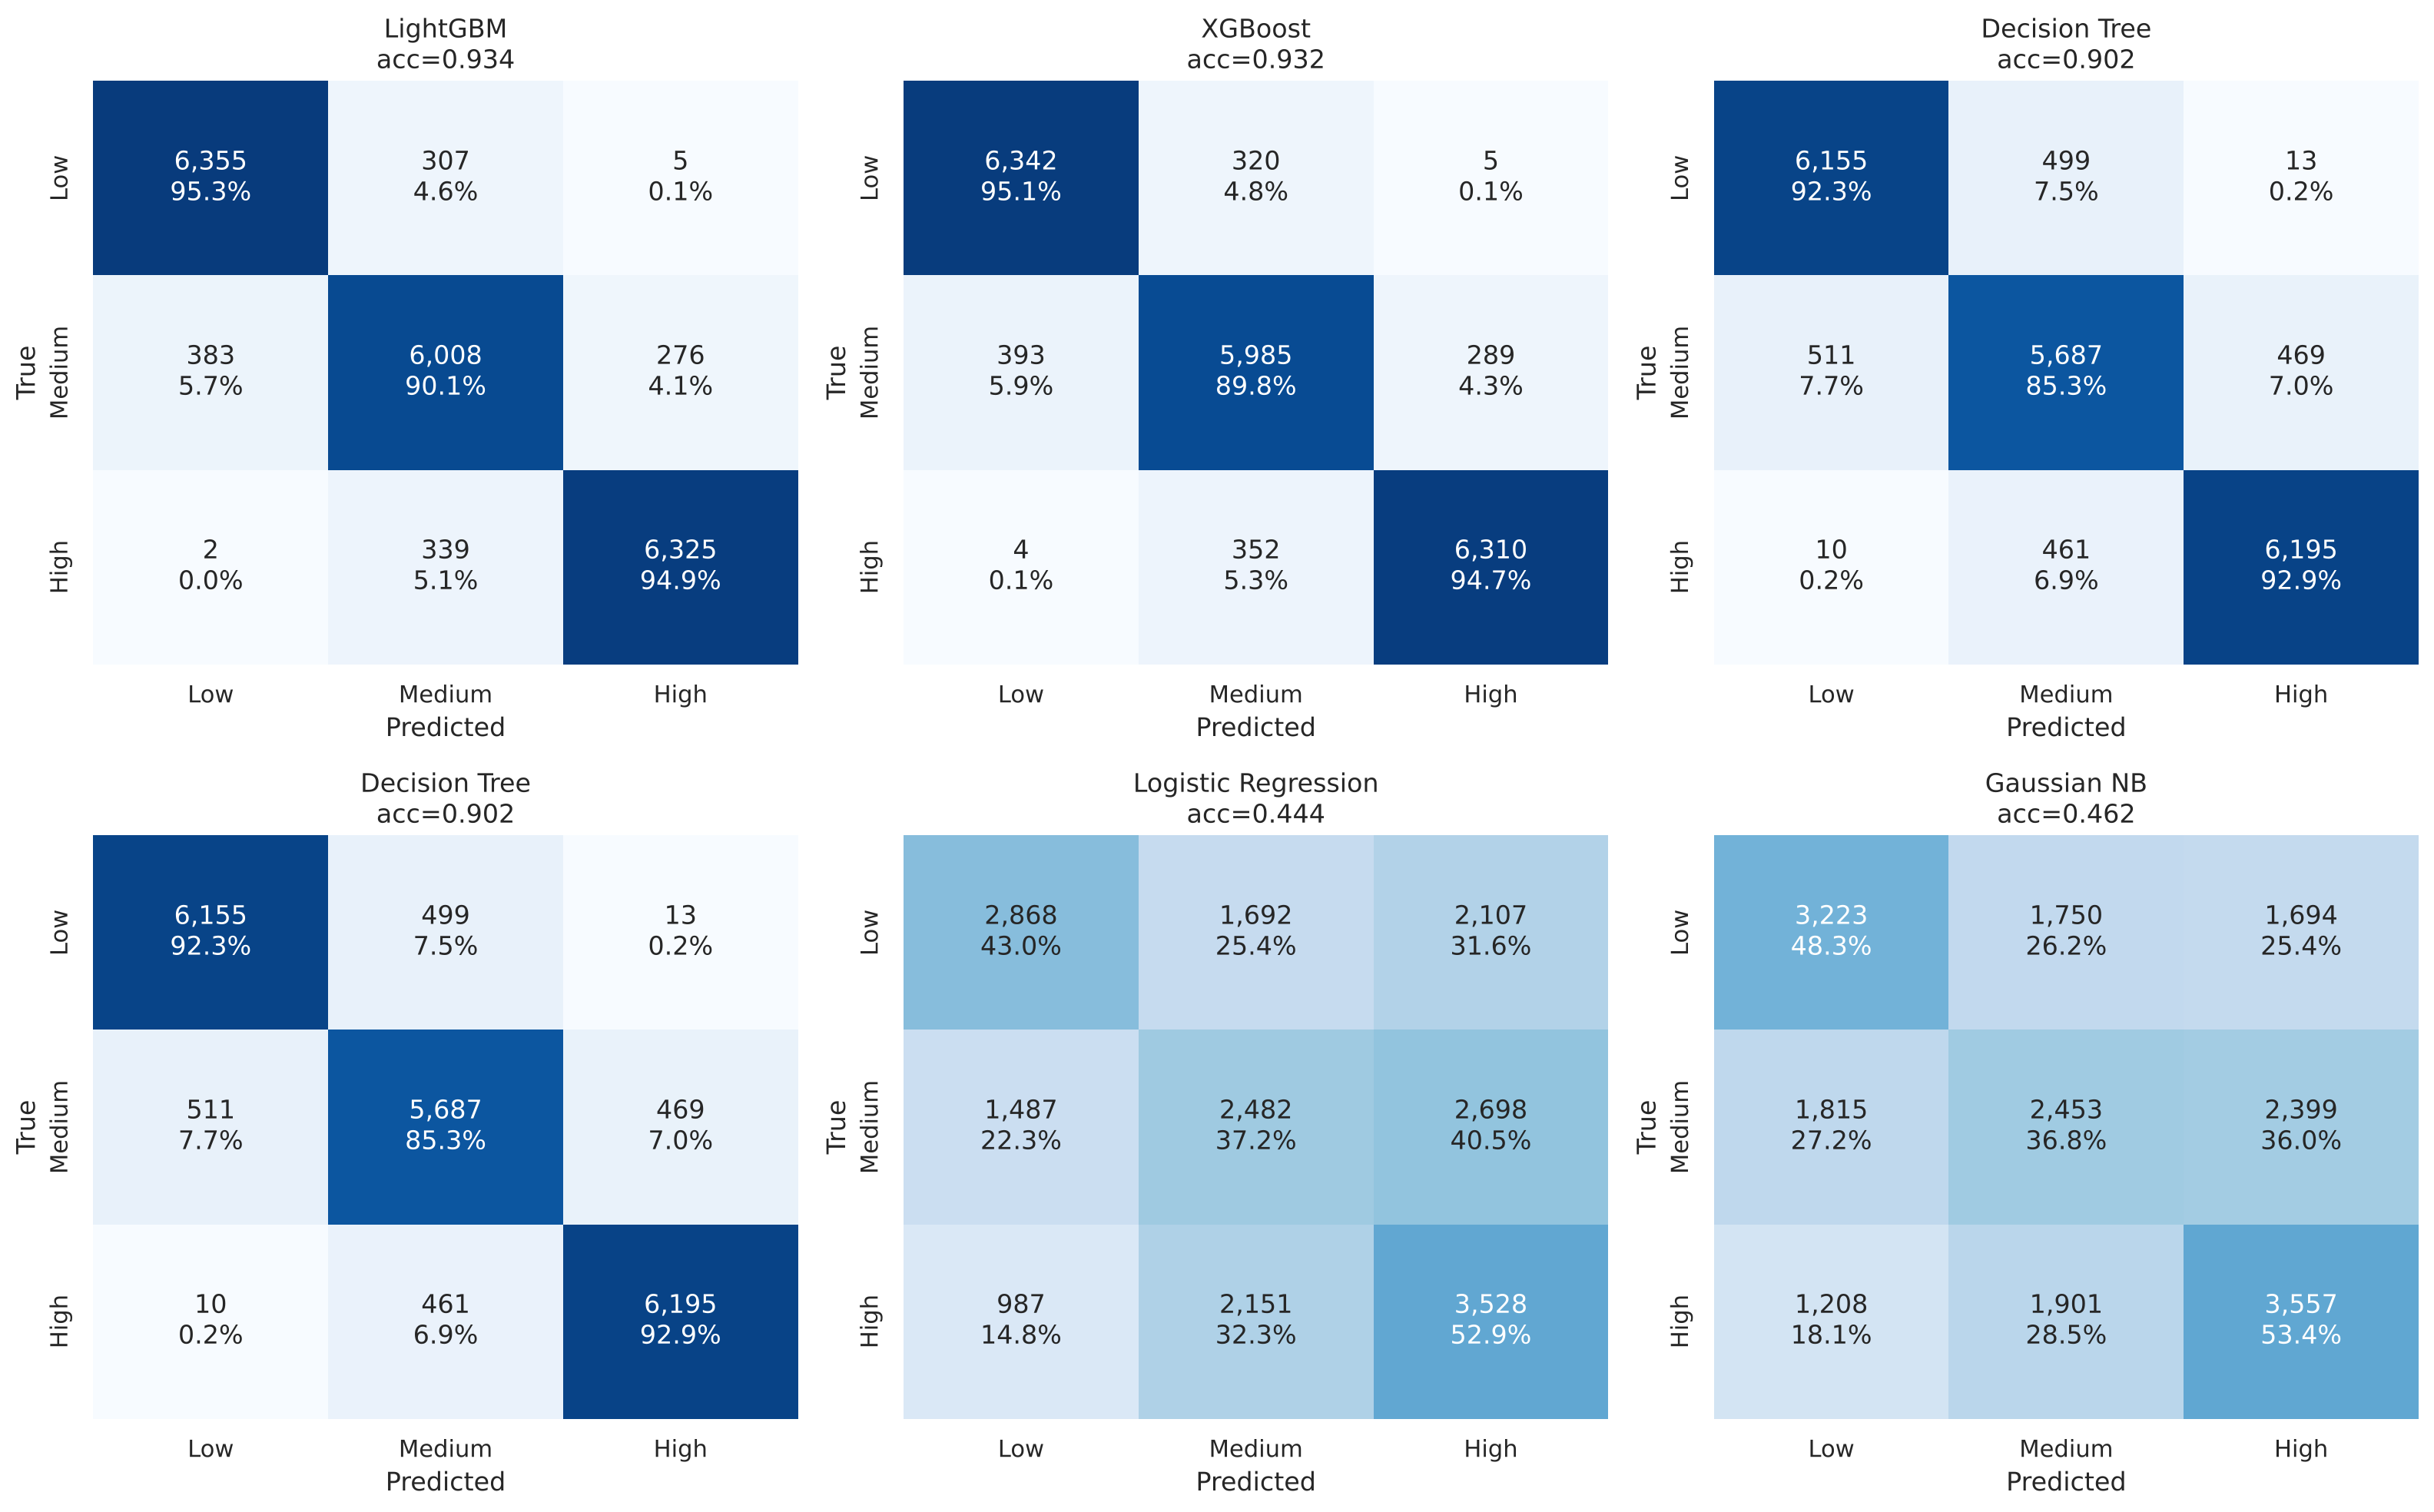
\includegraphics[width=0.9\textwidth]{figures/13_confusion_matrices.png}
\caption{Test-set confusion matrices (counts and row percentages). Top: the three best models. Bottom: the unpruned decision tree and two under-fitting linear/probabilistic models.}
\label{fig:cm}
\end{figure*}

\begin{table}[!t]
\caption{Interpretation of the confusion matrices (test set, 20{,}000 rows)}
\label{tab:cmint}
\centering
\setlength{\tabcolsep}{2.5pt}
\begin{tabular}{lccccc}
\toprule
 & \multicolumn{3}{c}{Recall (L / M / H)} & Errors & Far (L$\leftrightarrow$H) \\
\midrule
LightGBM & 0.953 & 0.901 & 0.949 & 1{,}312 & 7 (0.5\%) \\
XGBoost & 0.951 & 0.898 & 0.947 & 1{,}363 & 9 (0.7\%) \\
Decision Tree & 0.923 & 0.853 & 0.929 & 1{,}963 & 23 (1.2\%) \\
Gaussian NB & 0.483 & 0.368 & 0.534 & 10{,}767 & 2{,}902 (26.9\%) \\
Logistic Reg. & 0.430 & 0.372 & 0.529 & 11{,}122 & 3{,}094 (27.8\%) \\
\bottomrule
\end{tabular}
\end{table}

\subsection{ROC analysis}
Fig.~\ref{fig:roc} shows the one-vs-rest ROC curves of LightGBM (left) and the micro-averaged ROC curves of all nine models (right). The per-class AUCs of LightGBM are 0.995 (Low vs.\ rest), 0.982 (Medium vs.\ rest) and 0.996 (High vs.\ rest). This matches the confusion-matrix finding that the middle class is the hardest to isolate. The ranking of the models by AUC follows their ranking by accuracy, with one notable exception: the random forest and the MLP have modest accuracies (67--69\%) but respectable AUCs (0.850 and 0.852). Their probability \emph{rankings} are therefore much better than their hard decisions, a sign that their errors are concentrated near the decision thresholds.

\begin{figure*}[!t]
\centering
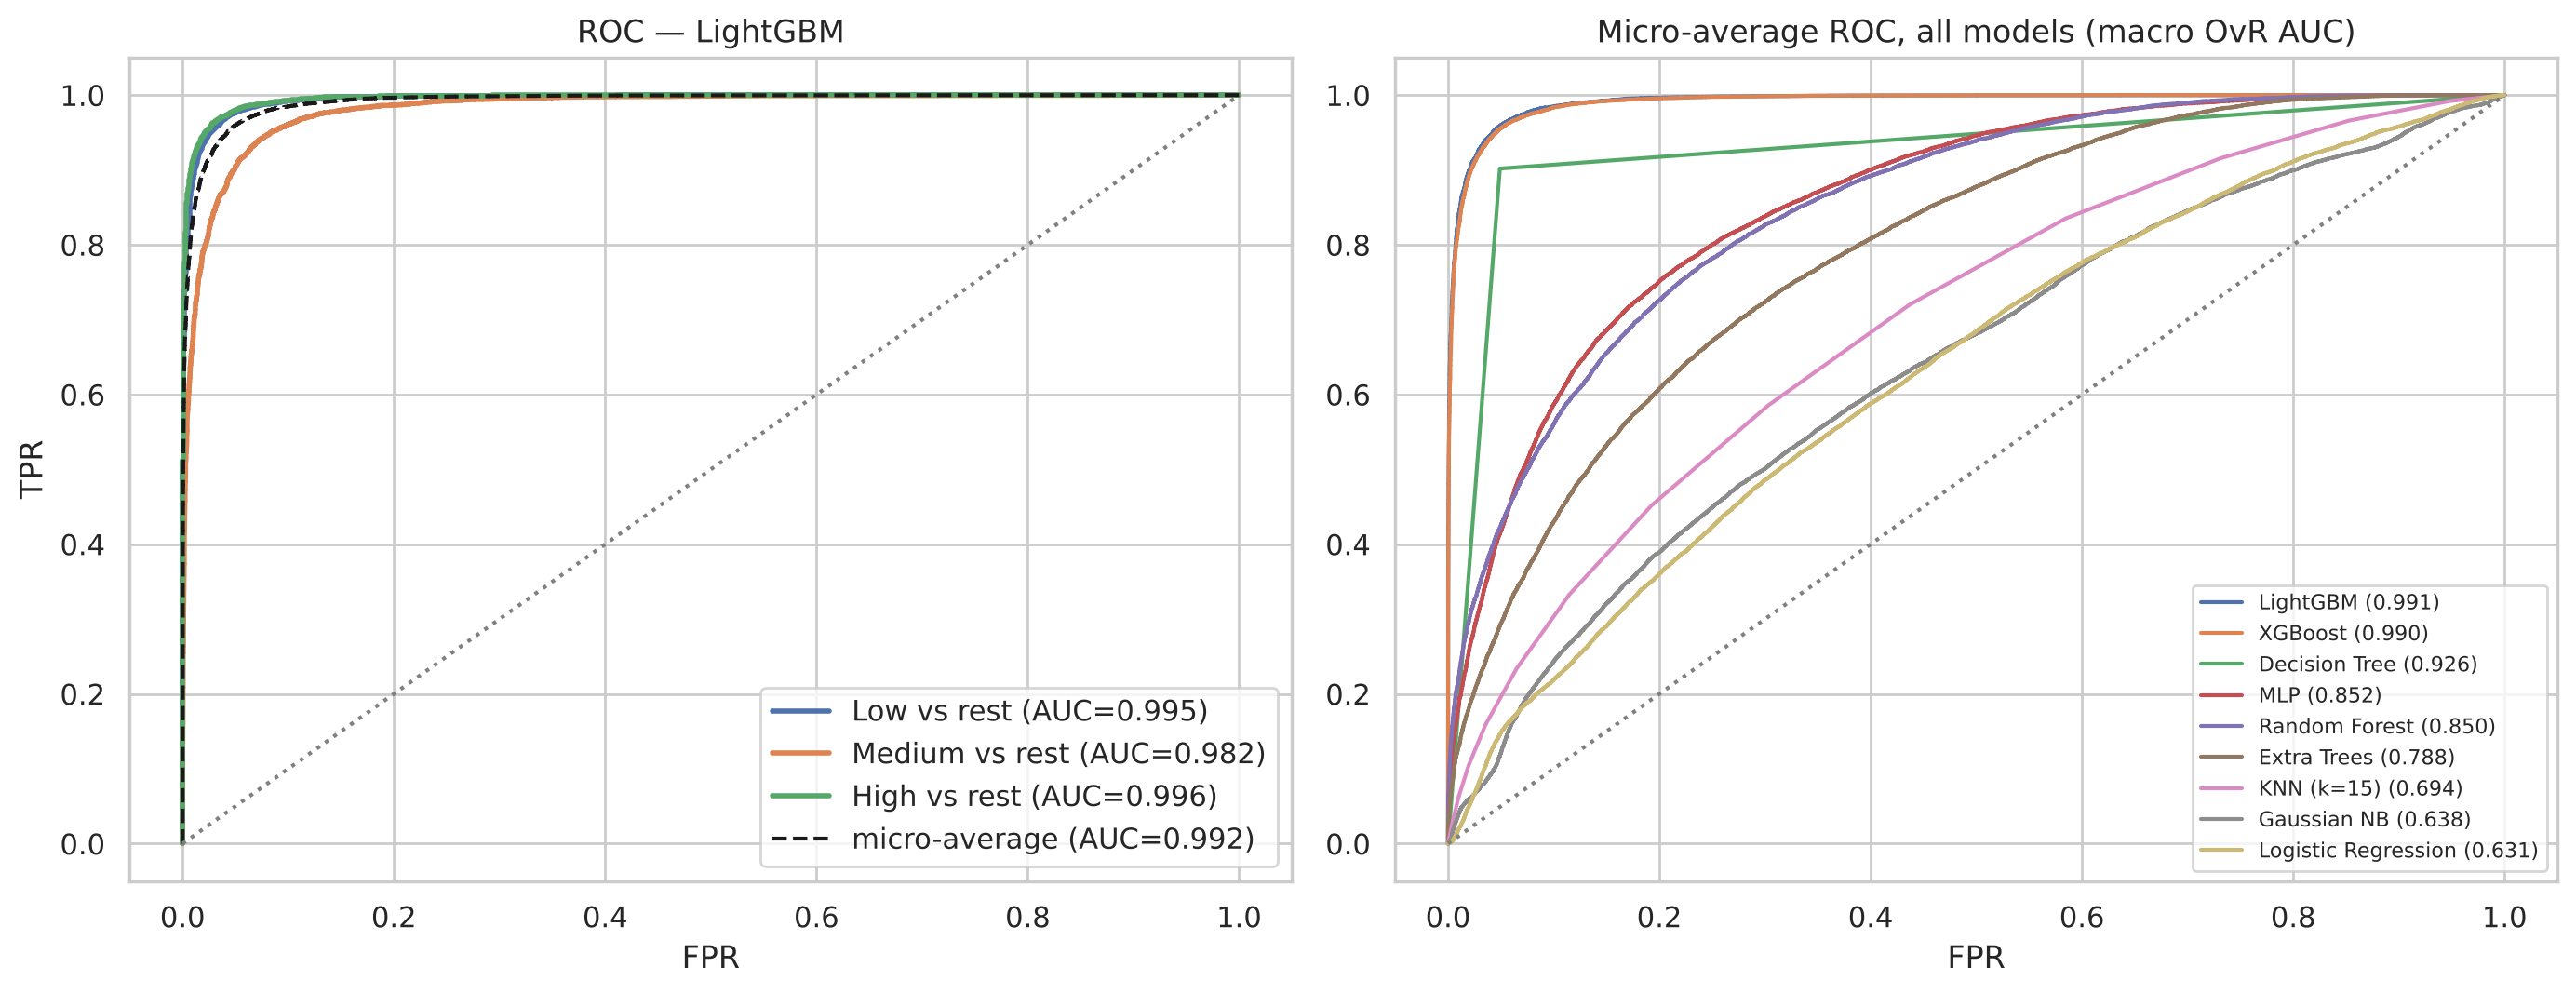
\includegraphics[width=0.9\textwidth]{figures/14_roc_curves.png}
\caption{ROC curves. Left: LightGBM, one-vs-rest per class and micro-average. Right: micro-averaged ROC of all models, with their macro one-vs-rest AUC in the legend.}
\label{fig:roc}
\end{figure*}

\subsection{Over-fitting and under-fitting}
Fig.~\ref{fig:fit} analyses the bias--variance behaviour from three angles.

\emph{Train--test gap} (left panel). Logistic regression and naive Bayes have train and test accuracies that are equal (gaps of $-0.3$ and $-0.6$ points) and both low: pure \textbf{under-fitting} (high bias). The unpruned decision tree is the textbook \textbf{over-fitting} case, with 100\% training accuracy and a 9.8-point gap. The random forest and extra trees show the most severe over-fitting, with gaps of 25.4 and 30.9 points. $k$-NN combines both problems: a low test accuracy (50.8\%) \emph{and} an 8.4-point gap, because with $k=15$ it memorises local neighbourhoods that are dominated by the noisy context variables. LightGBM and XGBoost have moderate gaps (5.9 and 5.6 points) just above our 5-point threshold. Their \emph{test} accuracy is nevertheless the best, so this is benign over-fitting typical of boosted ensembles, not a reason for concern.

\emph{Learning curve of LightGBM} (middle panel). Training accuracy stays at 100\% (99.8\% at full size) while validation accuracy rises steadily from 77.2\% with 2{,}666 rows to 85.5\%, 89.1\%, 91.5\% and 92.6\% with 53{,}333 rows, without plateauing. The remaining gap is therefore a \emph{variance} gap that more data would continue to close: the model has enough capacity, and its limiting factor is the number of examples per store-department combination ($45\times81$ cells with only a few dozen weeks each).

\emph{Validation curve of the decision-tree depth} (right panel). This curve shows the full transition from under- to over-fitting. At depth 2 training and validation accuracies are both 46.9\% (under-fitting). They rise together until depth 8 (76.6\% vs.\ 76.0\%). The validation accuracy peaks at \textbf{depth 16} (89.5\%), and beyond that the training accuracy keeps rising to 100\% while the validation accuracy declines slightly to 89.2\% (over-fitting).

\begin{figure*}[!t]
\centering
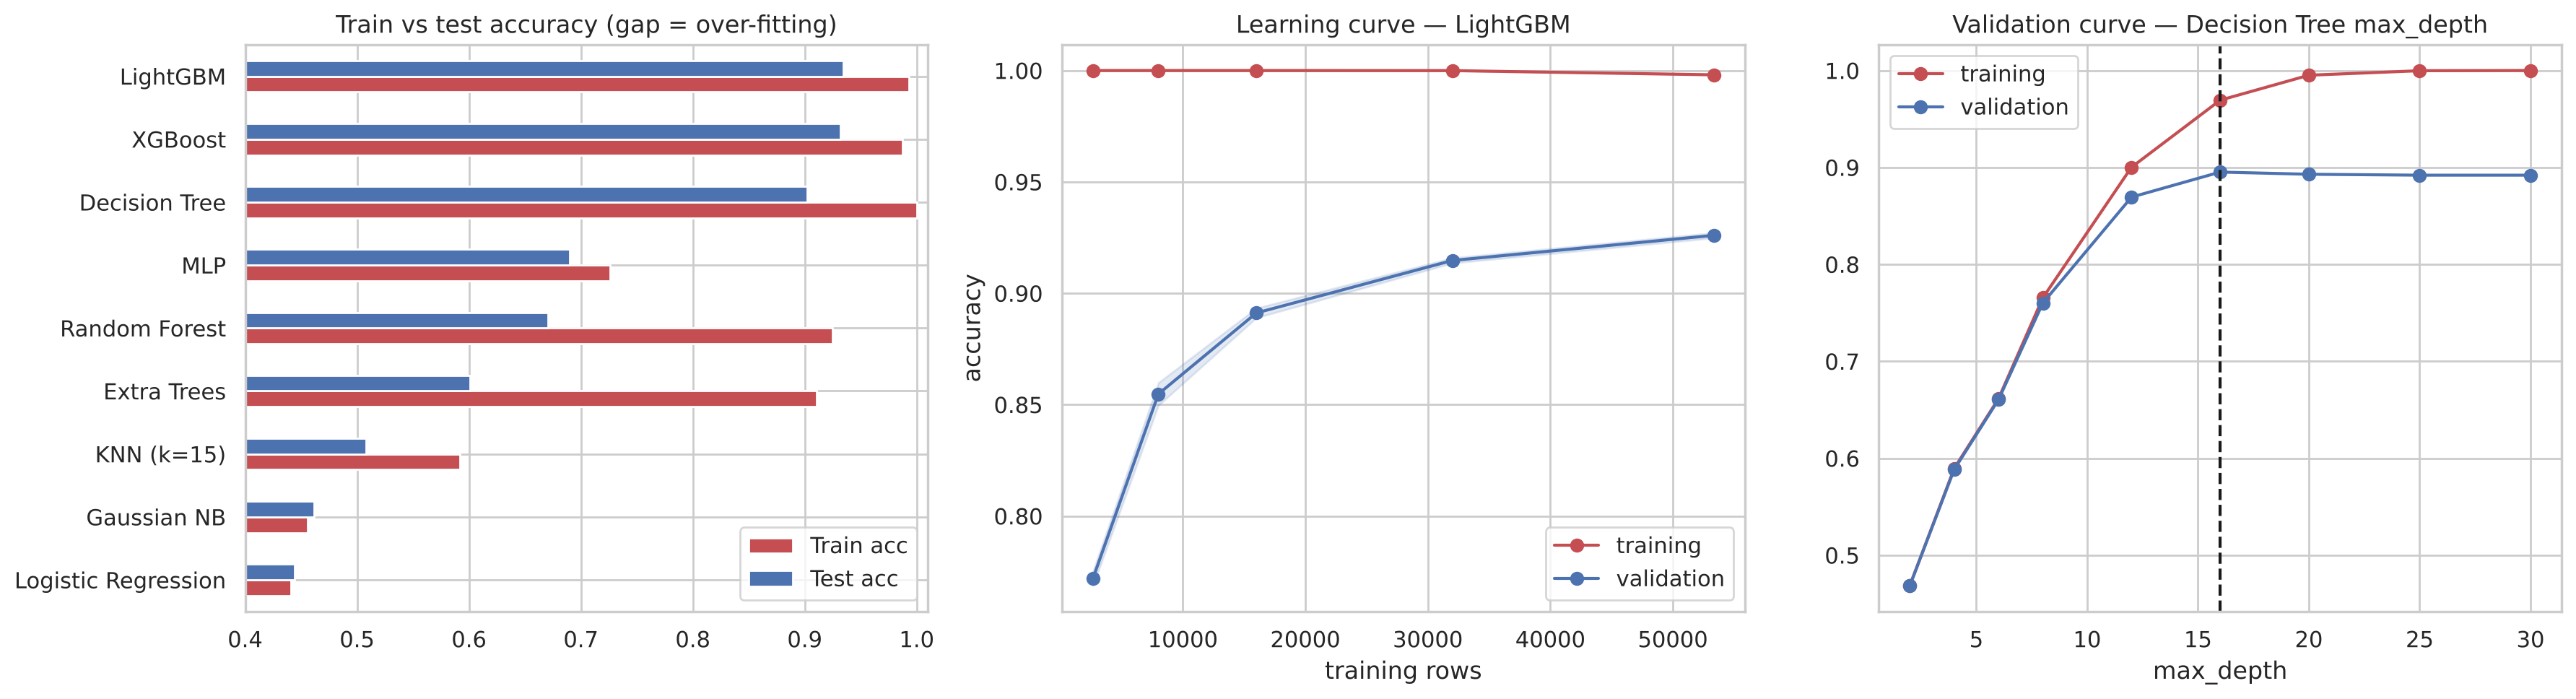
\includegraphics[width=\textwidth]{figures/15_over_under_fitting.png}
\caption{Over-/under-fitting analysis. Left: train vs.\ test accuracy of every model. Middle: learning curve of LightGBM (3-fold, mean $\pm$ std). Right: validation curve of the decision-tree depth, with the optimum at depth 16.}
\label{fig:fit}
\end{figure*}

\subsection{Ablation: why the default forests fail}\label{sec:res:ablation}
The poor results of the random forest (67.1\%) and extra trees (60.1\%) are surprising, given that a single unpruned tree reaches 90.2\%. We hypothesised that the cause is the default \texttt{max\_features}$=\sqrt{d}$. With $d=25$, each split may only consider 5 randomly drawn features, so the dominant \texttt{Dept} variable (67\% of LightGBM's gain) is available at only about 20\% of the splits. The trees are then forced to split on store-week context variables (\texttt{CPI}, \texttt{Temperature}, \texttt{Fuel\_Price}), which are almost unique per store-week and let the trees memorise the training data --- hence the very large train--test gaps.

Table~\ref{tab:ablation} confirms the hypothesis. Raising \texttt{max\_features} to 50\% of the features lifts the random forest from 67.1\% to 91.4\% and extra trees from 60.1\% to 90.5\%. Letting every split see all features (plain bagging) brings them to \textbf{93.0\%} and \textbf{93.3\%}, within 0.2 points of LightGBM, while the train--test gaps shrink from 25--31 points to 3--6 points. The general lesson for mixed-type tabular data is that the random-subspace mechanism, which normally decorrelates trees, becomes harmful when one feature carries most of the signal. The ``failure'' of the default forests is thus a hyper-parameter effect, not a limitation of bagging itself.

\begin{table}[!t]
\caption{Effect of \texttt{max\_features} on the forests (150 trees, minimum leaf 2; same 80/20 split)}
\label{tab:ablation}
\centering
\begin{tabular}{llcccc}
\toprule
Model & max\_feat. & Train & Test & F1 & AUC \\
\midrule
Random Forest & $\sqrt{d}$ (5) & 0.925 & 0.671 & 0.670 & 0.850 \\
 & 0.5 (12) & 0.990 & 0.914 & 0.914 & 0.981 \\
 & 1.0 (25) & 0.989 & \textbf{0.930} & \textbf{0.930} & \textbf{0.988} \\
\midrule
Extra Trees & $\sqrt{d}$ (5) & 0.910 & 0.601 & 0.599 & 0.788 \\
 & 0.5 (12) & 0.998 & 0.905 & 0.905 & 0.977 \\
 & 1.0 (25) & 0.997 & \textbf{0.933} & \textbf{0.933} & \textbf{0.990} \\
\bottomrule
\end{tabular}
\end{table}


\subsection{Effect of reduction and selection on the best model}\label{sec:res:subsets}
Finally, LightGBM was retrained on every selected subset and on three linear projections, using the same 80/20 split (Table~\ref{tab:subsets}, Fig.~\ref{fig:subsets}). Three results stand out.

\begin{enumerate}
\item \textbf{Metaheuristic subsets are the best.} The 6-feature GA subset gives the highest test accuracy of all inputs (\textbf{93.70\%}, F1 0.9369, AUC 0.9915), slightly \emph{above} the full 25-feature model (93.44\%). It does so with 76\% fewer features and 42\% less training time (5.5\,s vs.\ 9.5\,s). BPSO (9 features) is second (93.64\%). SA, with only 5 features, retains 99.8\% of the full model's accuracy (93.22\%). Removing noise variables thus reduces over-fitting as well as cost: the GA model's train--test gap falls to 4.5 points, below the 5-point threshold.
\item \textbf{Non-linear wrappers and embedded selectors are close behind; linear embedded and filter subsets lose accuracy.} RFE (93.54\%), LightGBM-gain (93.46\%) and both SFS variants (93.3--93.4\%) match the full model with 10 features. The L2 subset (91.46\%) and the filter subset (91.04\%) lose 2--2.4 points, because they were chosen by linear or univariate criteria that over-rate the redundant store-type dummies and miss interactions.
\item \textbf{Projections destroy the signal the trees need.} LightGBM on the 16 PCA (or SVD) components drops to 69.7\% accuracy, and on the 2 LDA axes to 51.1\% --- losses of 24 and 42 points. Rotating the data mixes the decisive nominal \texttt{Dept} variable with continuous noise, so the axis-aligned splits that make trees effective are no longer possible. For tree ensembles on mixed-type tabular data, \emph{selection} is clearly preferable to \emph{reduction}.
\end{enumerate}

\begin{table*}[!t]
\caption{LightGBM re-trained on each feature subset or projection (80{,}000 train / 20{,}000 test rows)}
\label{tab:subsets}
\centering
\begin{tabular}{lcccccc}
\toprule
Input & \# dims & Train acc. & Test acc. & Macro-F1 & ROC-AUC & Fit (s) \\
\midrule
GA (metaheuristic) & 6 & 0.9823 & \textbf{0.9370} & \textbf{0.9369} & \textbf{0.9915} & 5.5 \\
BPSO (metaheuristic) & 9 & 0.9826 & 0.9364 & 0.9364 & 0.9915 & 5.7 \\
RFE (wrapper) & 10 & 0.9922 & 0.9354 & 0.9354 & 0.9910 & 6.2 \\
LightGBM gain (embedded) & 10 & 0.9907 & 0.9346 & 0.9346 & 0.9911 & 6.6 \\
All features & 25 & 0.9929 & 0.9344 & 0.9344 & 0.9906 & 9.5 \\
SFS backward (wrapper) & 10 & 0.9864 & 0.9342 & 0.9342 & 0.9909 & 7.2 \\
SFS forward (wrapper) & 10 & 0.9695 & 0.9332 & 0.9332 & 0.9907 & 5.1 \\
Elastic-Net (embedded) & 21 & 0.9921 & 0.9330 & 0.9330 & 0.9903 & 8.4 \\
SA (metaheuristic) & 5 & 0.9695 & 0.9322 & 0.9322 & 0.9907 & 5.0 \\
L1 / Lasso (embedded) & 19 & 0.9920 & 0.9322 & 0.9322 & 0.9903 & 8.4 \\
L2 / Ridge (embedded) & 10 & 0.9569 & 0.9146 & 0.9146 & 0.9859 & 5.3 \\
Filter, rank fusion & 10 & 0.9622 & 0.9104 & 0.9103 & 0.9841 & 6.2 \\
PCA, 16 comp.\ (95\% var.) & 16 & 0.9017 & 0.6968 & 0.6960 & 0.8761 & 9.5 \\
SVD, 16 comp. & 16 & 0.9017 & 0.6968 & 0.6960 & 0.8761 & 9.9 \\
LDA, 2 axes & 2 & 0.6018 & 0.5108 & 0.5104 & 0.6984 & 4.5 \\
\bottomrule
\end{tabular}
\end{table*}


\begin{figure}[!t]
\centering
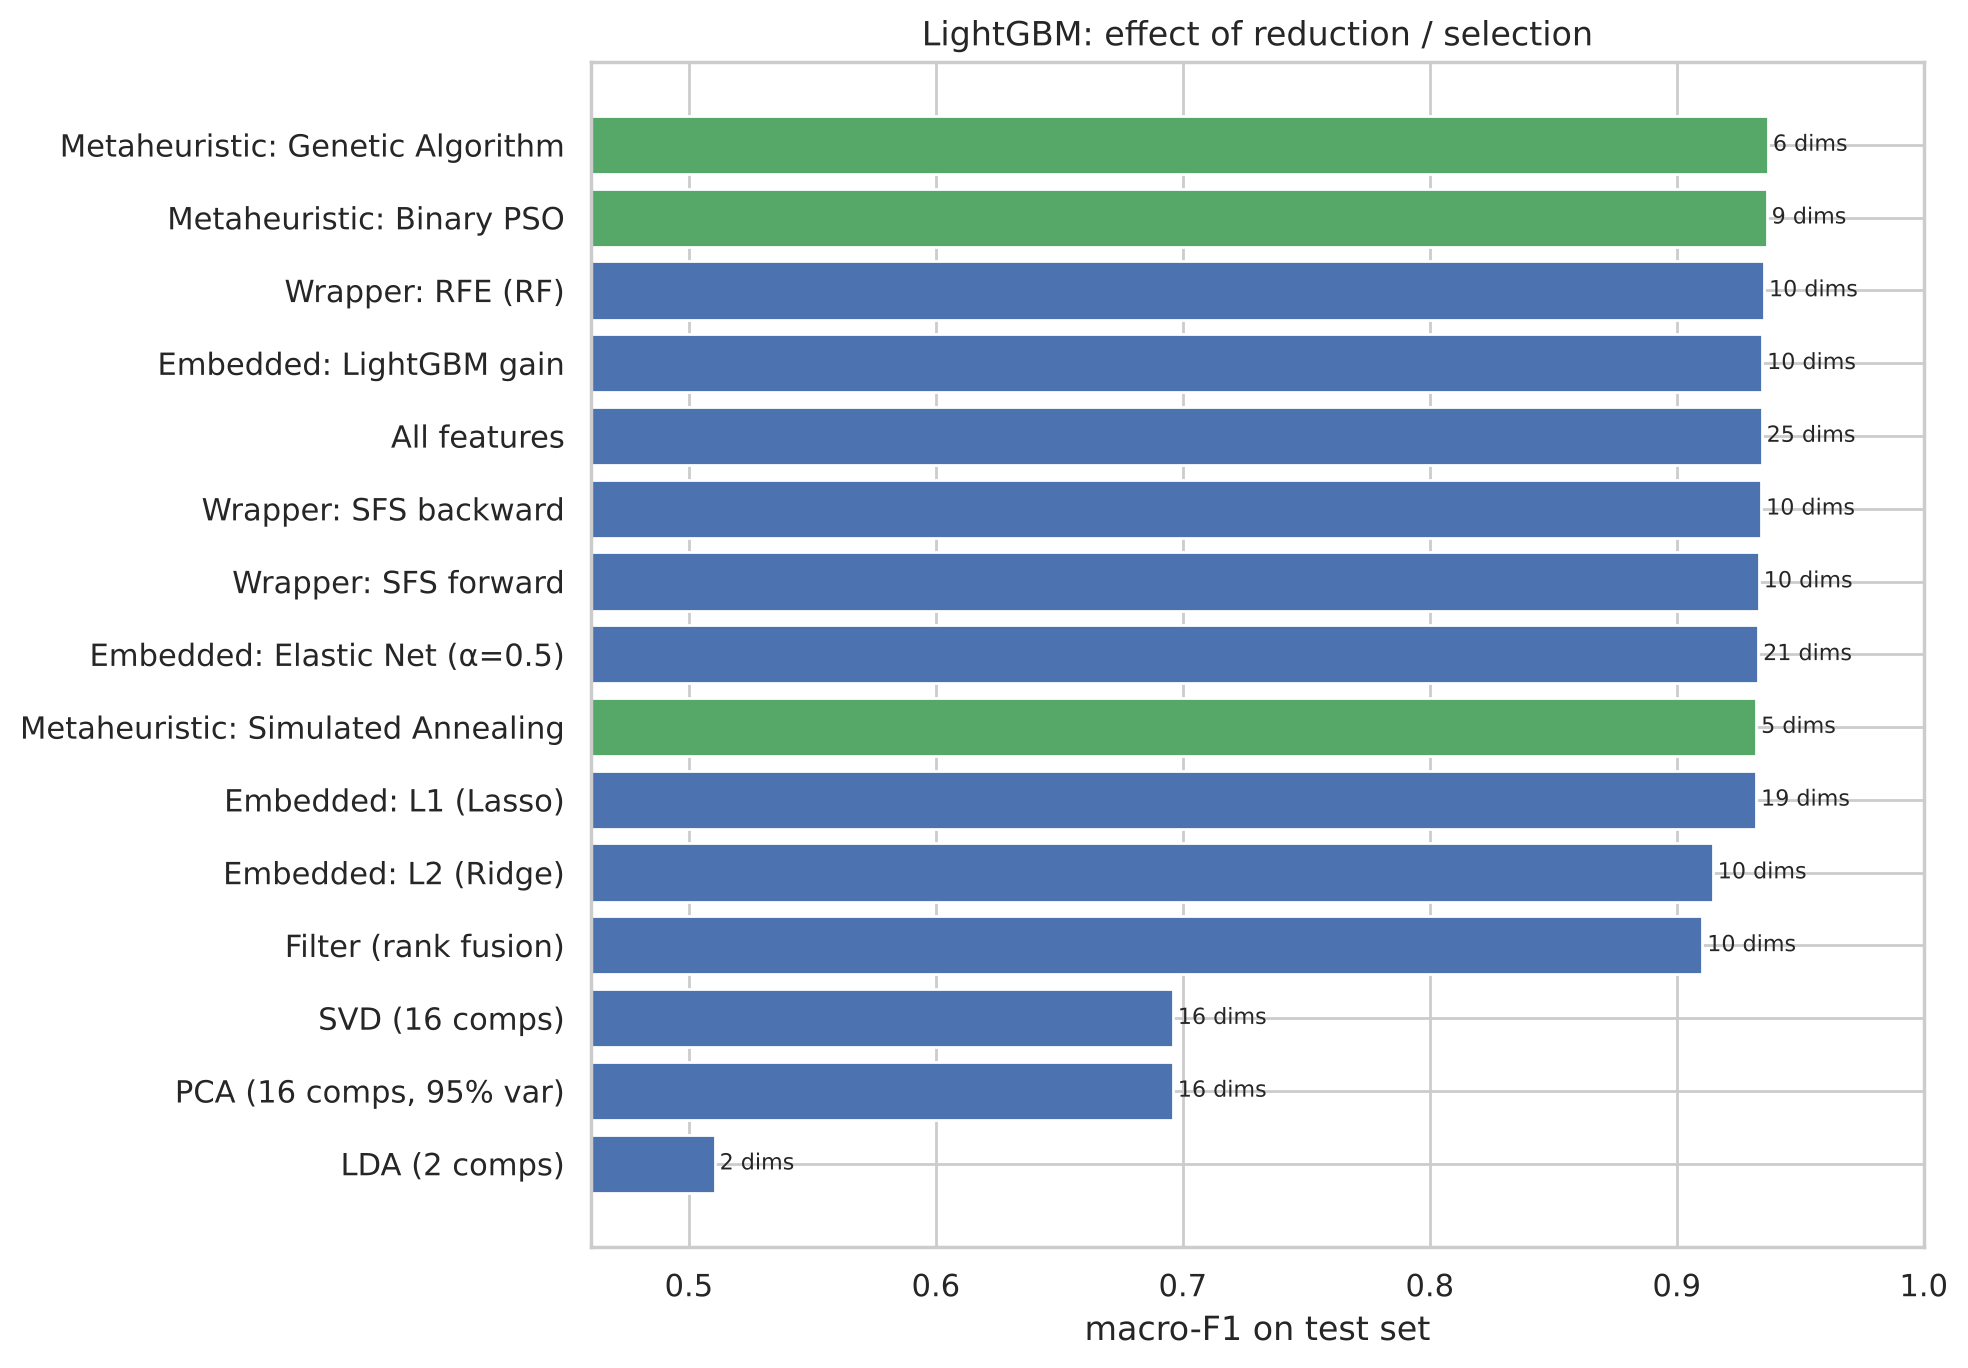
\includegraphics[width=\columnwidth]{figures/16_subset_comparison.png}
\caption{Test macro-F1 of LightGBM for every feature subset and projection (number of input dimensions annotated). Metaheuristic subsets are shown in green.}
\label{fig:subsets}
\end{figure}
